\chapter{FLOATING POINT COMPRESSION}
\label{chapter:fzip}
\newif\ifshort

%\shortfalse
%or
\shorttrue

\newif\ifbwtsec

\bwtsecfalse
%\bwtsectrue
Floating point compression is the second half of matrix compression. Figure \ref{tbl:value} shows a comparison of compression schemes. In the end, we created a program (and library) called fzip. In total fzip takes advantage of three compressible features of datasets: repeating sequences of values (patterns larger than 8 bytes long), repeating values (patterns exactly 8 bytes long), and repeating prefixes (patterns less than 8 bytes long).

For SpMV we need to make a hardware decoder. Currently everything except the BWT should be hardware amenable. We can remove that part and still expect good compression. Removing BWT removes compressing patterns larger than 8 bytes long. In the future we could use methods like LZW \cite{}, which is a little bit easier to get into hardware.
\begin{table*}
\centering
\begin{threeparttable}
\caption{Detailed value compression analysis and performance comparison}
\label{tbl:value}
\begin{tabular}{ccccccccc}
\hline
\bfseries Matrix & \bfseries \tikz \node[rotate=90]{uncompressed}; & \bfseries \tikz \node[rotate=90]{Unique Values}; & \bfseries \tikz \node[rotate=90]{Unique/nnz $\times 8$}; & \bfseries \tikz \node[rotate=90]{256 Common}; & \bfseries \tikz \node[rotate=90]{GZIP}; & \bfseries \tikz \node[rotate=90]{FPC}; & \bfseries \tikz \node[rotate=90]{\shortstack{Pattern\\ Compression\\ Unlimited}}; & \bfseries \tikz \node[rotate=90]{\shortstack{Pattern\\ Compression\\ 32KB}};\\
\hline
dense2\tnote{a} & $8.00$ & $1.00$ & $0.00$ & $1.00$ & $0.01$ & $0.50$ & $0.75$ & $0.76$ \\
pdb1HYS & $8.00$ & $1.10 \times 10^{6}$ & $4.08$ & $7.99$ & $4.15$ & $7.99$ & $5.07$ & $7.91$ \\
consph & $8.00$ & $1.24 \times 10^{6}$ & $3.28$ & $7.99$ & $5.10$ & $7.95$ & $4.77$ & $7.91$ \\
cant & $8.00$ & $1.07 \times 10^{2}$ & $0.00$ & $1.00$ & $0.11$ & $0.91$ & $0.89$ & $0.90$ \\
pwtk & $8.00$ & $3.63 \times 10^{6}$ & $5.04$ & $7.95$ & $4.29$ & $7.37$ & $5.83$ & $7.81$ \\
rma10\tnote{a} & $8.00$ & $1.00$ & $0.00$ & $1.00$ & $0.01$ & $0.50$ & $0.75$ & $0.76$ \\
qcd5\_4\tnote{a} & $8.00$ & $1.00$ & $0.00$ & $1.00$ & $0.01$ & $0.50$ & $0.75$ & $0.77$ \\
shipsec1 & $8.00$ & $8.86 \times 10^{4}$ & $0.56$ & $6.39$ & $2.08$ & $3.80$ & $2.34$ & $4.06$ \\
mac\_econ\_fwd500 & $8.00$ & $1.08 \times 10^{5}$ & $1.36$ & $5.20$ & $0.73$ & $1.45$ & $2.32$ & $2.03$ \\
mc2depi & $8.00$ & $3.58 \times 10^{3}$ & $0.00$ & $4.94$ & $1.24$ & $5.01$ & $1.58$ & $1.51$ \\
cop20k\_A & $8.00$ & $9.56 \times 10^{5}$ & $5.84$ & $7.97$ & $5.53$ & $7.97$ & $5.92$ & $7.85$ \\
scircuit & $8.00$ & $8.82 \times 10^{4}$ & $1.44$ & $5.41$ & $1.95$ & $3.68$ & $2.61$ & $3.56$ \\
webbase-1M & $8.00$ & $5.65 \times 10^{2}$ & $0.00$ & $1.48$ & $0.38$ & $1.92$ & $1.10$ & $1.11$ \\
\hline
average\tnote{b} & $8.00$ & $7.22 \times 10^{5}$ & $2.16$ & $5.63$ & $2.56$ & $4.81$ & $3.24$ & $4.46$ \\

\hline
\end{tabular}
\begin{tablenotes}
\item [a] Boolean matrices
\item [b] Excludes boolean matrices
\end{tablenotes}
\end{threeparttable}
\end{table*}
%
\section{Previous work}
\label{sec:val}
It was noted in \cite{prelim:kourtis} that sparse matrices often have repeated values. This is the focus of our value compression. $R^3$ had a simple scheme using this. It stored the 256 most common values, so those common values could be represented as one byte. The performance of this scheme is shown in the column ``256 common" in table \ref{tbl:value}.\\
\indent Taking a step back, uncompressed data would take 8 bytes per element. Any compression scheme should take less than 8 bytes per element. We looked at \cite{smac:burtscher} describing it's own compression scheme FPC. FPC performs well. This scheme looks for repeated patterns. However it does not exploit the fact most of its compression comes from exact (8 byte) value repeats.\\
\indent Gzip performs quite well too. We have a general understanding of how Gzip works. We suspect the reason for the good performance is the large memory space and being able to look up previously occurring 8-byte values.\par
\indent Our focus on using repeated values is reinforced by looking at the number of unique values. If only the unique values were stored the average compression would be 2.16 bytes per element. This can not be used by itself since this ignores the indexing required to access these values, but this gives an estimate of the possible compression size.%
\indent In the remainder of this paper we talk about 
\ifshort
\else
previous approaches (section \ref{sec:relatedWork}), 
\fi
an analysis of floating point datasets (section \ref{sec:analysis}), our approach to floating point compression (section \ref{sec:approach}) and our results (section \ref{sec:results}).
\begin{figure}
\center
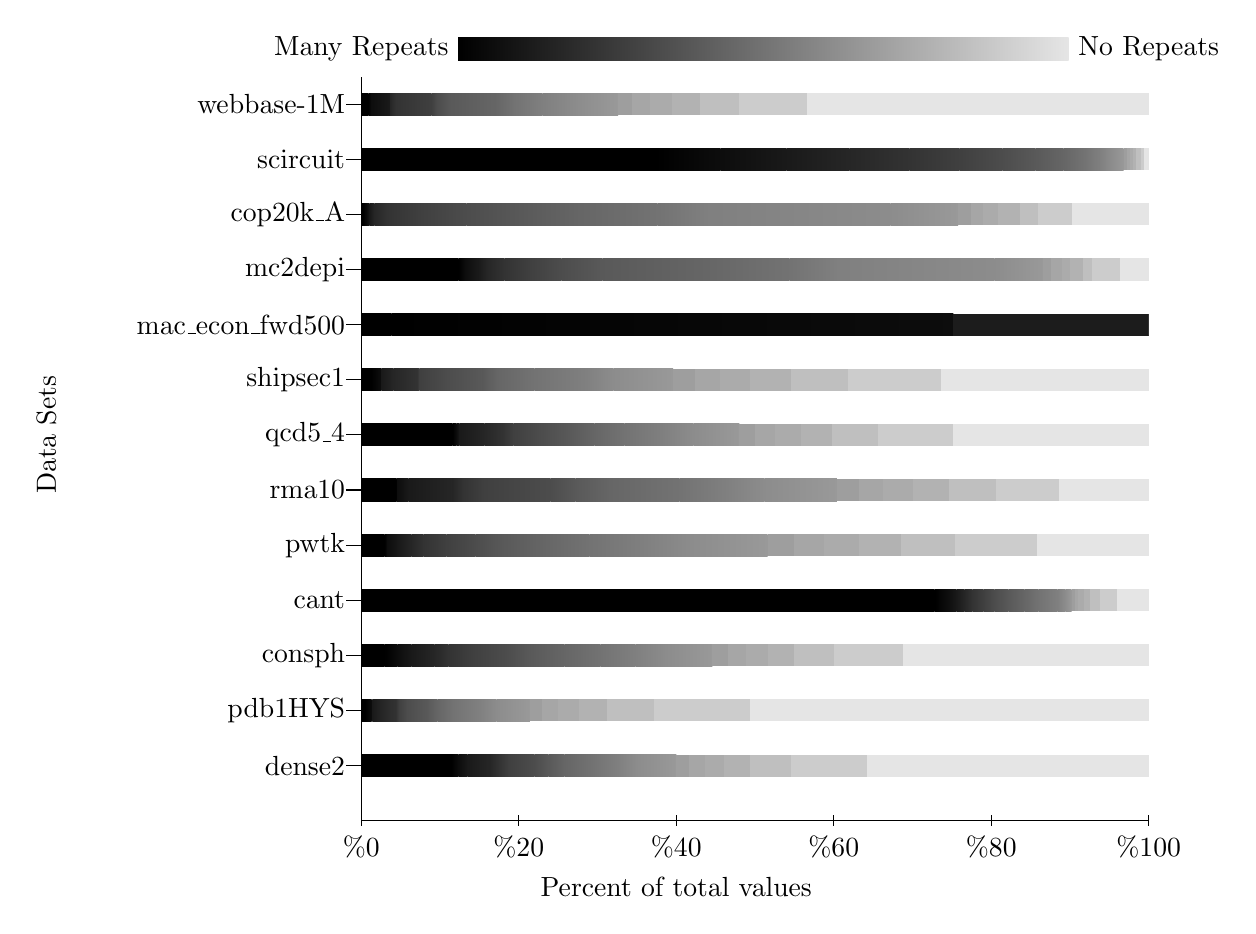
\begin{tikzpicture}[yscale=.7,xscale=2]

\path[draw] (0,0) -- (0,13.5);
\path[draw] (0,0) -- (5,0);
\foreach \x/\v in {0/0,1/20,2/40,3/60,4/80,5/100}{
    \draw (\x,.1) -- (\x,-.1)node[anchor=north]{\%\v};
}

\foreach \n/\y in {dense2/1, pdb1HYS/2, consph/3, cant/4, pwtk/5, rma10/6, qcd5\_4/7, shipsec1/8, mac\_econ\_fwd500/9, mc2depi/10, cop20k\_A/11, scircuit/12, webbase-1M/13}{
    \draw (.1,\y) -- (-.1,\y)node[anchor=east,rotate=0,inner sep=0]{\n};
}
\node at (2,-1.2){Percent of total values};
\node[rotate=90] at (-2,7){Data Sets};

%msg_bt
\foreach \xa/\xb/\sa/\sb in {0/0.571/100/100,0.571/0.617/100/95,0.617/0.675/95/90,0.675/0.816/90/85,0.816/0.875/85/80,0.875/0.937/80/75,0.937/1.1/75/70,1.1/1.19/70/65,1.19/1.29/65/60,1.29/1.47/60/55,1.47/1.63/55/50,1.63/1.75/50/45,1.75/2/45/40,}{
    \shade[left color=black!\sa,right color=black!\sb] (\xa,0.8) rectangle (\xb,1.2);
}
\foreach \xa/\xb/\s in {2/2.08/38,2.08/2.18/35,2.18/2.3/33,2.3/2.47/30,2.47/2.73/25,2.73/3.21/20,3.21/5/10}{
    \fill[black!\s] (\xa,0.8) rectangle (\xb,1.2);
}
%msg_lu
\foreach \xa/\xb/\sa/\sb in {0/0.0238/100/100,0.0238/0.0644/100/95,0.0644/0.0709/95/90,0.0709/0.13/90/85,0.13/0.22/85/80,0.22/0.238/80/75,0.238/0.29/75/70,0.29/0.417/70/65,0.417/0.485/65/60,0.485/0.582/60/55,0.582/0.747/55/50,0.747/0.859/50/45,0.859/1.07/45/40,}{
    \shade[left color=black!\sa,right color=black!\sb] (\xa,1.8) rectangle (\xb,2.2);
}
\foreach \xa/\xb/\s in {1.07/1.15/38,1.15/1.25/35,1.25/1.38/33,1.38/1.56/30,1.56/1.86/25,1.86/2.47/20,2.47/5/10}{
    \fill[black!\s] (\xa,1.8) rectangle (\xb,2.2);
}
%msg_sp
\foreach \xa/\xb/\sa/\sb in {0/0.147/100/100,0.147/0.231/100/95,0.231/0.318/95/90,0.318/0.464/90/85,0.464/0.554/85/80,0.554/0.709/80/75,0.709/0.924/75/70,0.924/1.07/70/65,1.07/1.29/65/60,1.29/1.52/60/55,1.52/1.74/55/50,1.74/1.94/50/45,1.94/2.23/45/40,}{
    \shade[left color=black!\sa,right color=black!\sb] (\xa,2.8) rectangle (\xb,3.2);
}
\foreach \xa/\xb/\s in {2.23/2.33/38,2.33/2.44/35,2.44/2.58/33,2.58/2.75/30,2.75/3/25,3/3.44/20,3.44/5/10}{
    \fill[black!\s] (\xa,2.8) rectangle (\xb,3.2);
}
%msg_sppm
\foreach \xa/\xb/\sa/\sb in {0/3.64/100/100,3.64/3.72/100/95,3.72/3.78/95/90,3.78/3.83/90/85,3.83/3.88/85/80,3.88/3.95/80/75,3.95/4.02/75/70,4.02/4.11/70/65,4.11/4.21/65/60,4.21/4.3/60/55,4.3/4.42/55/50,4.42/4.47/50/45,4.47/4.51/45/40,}{
    \shade[left color=black!\sa,right color=black!\sb] (\xa,3.8) rectangle (\xb,4.2);
}
\foreach \xa/\xb/\s in {4.51/4.53/38,4.53/4.55/35,4.55/4.59/33,4.59/4.63/30,4.63/4.69/25,4.69/4.8/20,4.8/5/10}{
    \fill[black!\s] (\xa,3.8) rectangle (\xb,4.2);
}
%msg_sweep3d
\foreach \xa/\xb/\sa/\sb in {0/0.148/100/100,0.148/0.164/100/95,0.164/0.238/95/90,0.238/0.32/90/85,0.32/0.396/85/80,0.396/0.541/80/75,0.541/0.726/75/70,0.726/0.9/70/65,0.9/1.16/65/60,1.16/1.45/60/55,1.45/1.79/55/50,1.79/2.1/50/45,2.1/2.58/45/40,}{
    \shade[left color=black!\sa,right color=black!\sb] (\xa,4.8) rectangle (\xb,5.2);
}
\foreach \xa/\xb/\s in {2.58/2.75/38,2.75/2.94/35,2.94/3.16/33,3.16/3.43/30,3.43/3.77/25,3.77/4.29/20,4.29/5/10}{
    \fill[black!\s] (\xa,4.8) rectangle (\xb,5.2);
}
%num_brain
\foreach \xa/\xb/\sa/\sb in {0/0.222/100/100,0.222/0.226/100/95,0.226/0.3/95/90,0.3/0.581/90/85,0.581/0.646/85/80,0.646/0.779/80/75,0.779/1.2/75/70,1.2/1.36/70/65,1.36/1.58/65/60,1.58/2.02/60/55,2.02/2.31/55/50,2.31/2.56/50/45,2.56/3.02/45/40,}{
    \shade[left color=black!\sa,right color=black!\sb] (\xa,5.8) rectangle (\xb,6.2);
}
\foreach \xa/\xb/\s in {3.02/3.16/38,3.16/3.31/35,3.31/3.5/33,3.5/3.73/30,3.73/4.03/25,4.03/4.43/20,4.43/5/10}{
    \fill[black!\s] (\xa,5.8) rectangle (\xb,6.2);
}
%num_comet
\foreach \xa/\xb/\sa/\sb in {0/0.58/100/100,0.58/0.604/100/95,0.604/0.625/95/90,0.625/0.783/90/85,0.783/0.899/85/80,0.899/0.965/80/75,0.965/1.14/75/70,1.14/1.32/70/65,1.32/1.48/65/60,1.48/1.67/60/55,1.67/1.91/55/50,1.91/2.11/50/45,2.11/2.4/45/40,}{
    \shade[left color=black!\sa,right color=black!\sb] (\xa,6.8) rectangle (\xb,7.2);
}
\foreach \xa/\xb/\s in {2.4/2.5/38,2.5/2.63/35,2.63/2.79/33,2.79/2.99/30,2.99/3.28/25,3.28/3.76/20,3.76/5/10}{
    \fill[black!\s] (\xa,6.8) rectangle (\xb,7.2);
}
%num_control
\foreach \xa/\xb/\sa/\sb in {0/0.0628/100/100,0.0628/0.119/100/95,0.119/0.128/95/90,0.128/0.205/90/85,0.205/0.353/85/80,0.353/0.37/80/75,0.37/0.544/75/70,0.544/0.772/70/65,0.772/0.862/65/60,0.862/1.1/60/55,1.1/1.42/55/50,1.42/1.6/50/45,1.6/1.98/45/40,}{
    \shade[left color=black!\sa,right color=black!\sb] (\xa,7.8) rectangle (\xb,8.2);
}
\foreach \xa/\xb/\s in {1.98/2.12/38,2.12/2.28/35,2.28/2.47/33,2.47/2.73/30,2.73/3.09/25,3.09/3.68/20,3.68/5/10}{
    \fill[black!\s] (\xa,7.8) rectangle (\xb,8.2);
}
%num_plasma
\foreach \xa/\xb/\sa/\sb in {0/0.191/100/100,0.191/3.76/100/95,3.76/3.76/95/90,}{
    \shade[left color=black!\sa,right color=black!\sb] (\xa,8.8) rectangle (\xb,9.2);
}
\foreach \xa/\xb/\s in {3.76/5/89,5/5/10}{
    \fill[black!\s] (\xa,8.8) rectangle (\xb,9.2);
}
%obs_error
\foreach \xa/\xb/\sa/\sb in {0/0.616/100/100,0.616/0.657/100/95,0.657/0.741/95/90,0.741/0.798/90/85,0.798/0.909/85/80,0.909/1.07/80/75,1.07/1.27/75/70,1.27/1.53/70/65,1.53/2.19/65/60,2.19/2.72/60/55,2.72/3.02/55/50,3.02/4.02/50/45,4.02/4.33/45/40,}{
    \shade[left color=black!\sa,right color=black!\sb] (\xa,9.8) rectangle (\xb,10.2);
}
\foreach \xa/\xb/\s in {4.33/4.38/38,4.38/4.45/35,4.45/4.5/33,4.5/4.58/30,4.58/4.64/25,4.64/4.82/20,4.82/5/10}{
    \fill[black!\s] (\xa,9.8) rectangle (\xb,10.2);
}
%obs_info
\foreach \xa/\xb/\sa/\sb in {0/0.0114/100/100,0.0114/0.0349/100/95,0.0349/0.053/95/90,0.053/0.0827/90/85,0.0827/0.164/85/80,0.164/0.38/80/75,0.38/0.667/75/70,0.667/1.02/70/65,1.02/1.39/65/60,1.39/1.88/60/55,1.88/2.2/55/50,2.2/3.36/50/45,3.36/3.79/45/40,}{
    \shade[left color=black!\sa,right color=black!\sb] (\xa,10.8) rectangle (\xb,11.2);
}
\foreach \xa/\xb/\s in {3.79/3.87/38,3.87/3.95/35,3.95/4.04/33,4.04/4.18/30,4.18/4.3/25,4.3/4.51/20,4.51/5/10}{
    \fill[black!\s] (\xa,10.8) rectangle (\xb,11.2);
}
%obs_spitzer
\foreach \xa/\xb/\sa/\sb in {0/1.87/100/100,1.87/2.28/100/95,2.28/2.7/95/90,2.7/3.1/90/85,3.1/3.48/85/80,3.48/3.8/80/75,3.8/4.07/75/70,4.07/4.28/70/65,4.28/4.46/65/60,4.46/4.59/60/55,4.59/4.69/55/50,4.69/4.76/50/45,4.76/4.84/45/40,}{
    \shade[left color=black!\sa,right color=black!\sb] (\xa,11.8) rectangle (\xb,12.2);
}
\foreach \xa/\xb/\s in {4.84/4.86/38,4.86/4.88/35,4.88/4.9/33,4.9/4.92/30,4.92/4.95/25,4.95/4.97/20,4.97/5/10}{
    \fill[black!\s] (\xa,11.8) rectangle (\xb,12.2);
}
%obs_temp
\foreach \xa/\xb/\sa/\sb in {0/0.0457/100/100,0.0457/0.0601/100/95,0.0601/0.177/95/90,0.177/0.182/90/85,0.182/0.22/85/80,0.22/0.446/80/75,0.446/0.482/75/70,0.482/0.563/70/65,0.563/0.855/65/60,0.855/0.971/60/55,0.971/1.15/55/50,1.15/1.37/50/45,1.37/1.63/45/40,}{
    \shade[left color=black!\sa,right color=black!\sb] (\xa,12.8) rectangle (\xb,13.2);
}
\foreach \xa/\xb/\s in {1.63/1.72/38,1.72/1.83/35,1.83/1.97/33,1.97/2.15/30,2.15/2.4/25,2.4/2.83/20,2.83/5/10}{
    \fill[black!\s] (\xa,12.8) rectangle (\xb,13.2);
}

%key
\node[fill=white] at (0,14)(high){Many Repeats};
\node[fill=white] at (5,14)(low){No Repeats};
\shade[left color=black,right color=black!10] ([yshift=-.2cm]high.east) rectangle ([yshift=.2cm]low.west);

\end{tikzpicture}
\caption[not robust]{The above figure shows the distribution of repeats in each dataset. Each shade represents a different number of repeats. For instance: \tikz \fill (0,0) rectangle (.2,.2);:$>512$, \tikz \fill[black!50] (0,0) rectangle (.2,.2);:$16$, \tikz \fill[black!20] (0,0) rectangle (.2,.2);:$2$, \tikz \fill[black!10] (0,0) rectangle (.2,.2);:$1$(no repeats).}
\label{fig:repeat}
\end{figure}
\section{Related Work}
\label{sec:relatedWork}
FPC, the program most similar to our work, uses predictors to compress data. A predictor uses the previous data in the data set to guess the current element in the data set. FPC uses hash functions to implement their predictors. Passing an argument between 1 and 25 to FPC configures the hash table size. Larger hash tables necessarily predict better because values in the hash table get overwritten less often. However, large hash tables cause slower performance compared to hash tables that can fit in cache.\\
\indent In FPC, each value gets encoded with a 4 bit header followed by 0, 1, 2, 3, 4, 6, 7 or 8 bytes. The first bit specifies which of the 2 predictors resulted in the most matching bytes compared to the correct current value. Then, the next 3 bits encode this number of bytes, however, 5 bytes is rounded down to 4 bytes. Then, the least significant bytes that the hash failed to predict follow.\\
\indent FPC has the advantage of speed. Particularly when the hash table fits in cache. Although good, the compression ratio suffers because predictors do not always get the best or a good prediction. If a pattern does not exist among the values in the data set then FPC can not predict with any accuracy. Let us design this ``anti-FPC" dataset. Take the set of numbers $\{10^0, 10^1, 10^2, 10^3, \dots, 10^9\}$ and randomly choose one (with replacement) to add to the anti-FPC dataset. We do this a million times to get a dataset with a million values (8MB in size). You can observe the performance of this in \figurename~\ref{fig:antiFpc}.\\
\begin{figure}
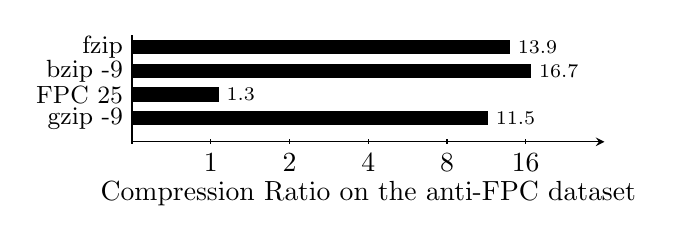
\begin{tikzpicture}[yscale=.3]
\draw (0,0) -- (0,4.5);
\draw[-stealth] (0,0) -- (6,0);
\foreach \x/\n in {0/,1/1,2/2,3/4,4/8,5/16}{
    \draw (\x,.1) -- (\x,-.1)node[anchor=north]{\n};
}
\node at (3,-2.2){Compression Ratio on the anti-FPC dataset};
\small
\foreach \y/\n in {0/,1/gzip -9,2/FPC 25,3/bzip -9,4/fzip}{
    \node[anchor=east, rotate=0] at (0,\y){\n};
}
\scriptsize
\foreach \x/\y/\n in {4.52/1/11.5,1.1/2/1.3,5.07/3/16.7,4.8/4/13.9}{
    \fill (0,\y-.3) rectangle (\x,\y+.3);
    \node[anchor=west] at (\x,\y){\n};
}
\end{tikzpicture}
\caption{We engineering a dataset to make the performance of FPC look bad compared to other programs. Although unfair, this shows a type of pattern that FPC does not exploit and other programs do. This problem exists because FPC only uses predictors for compression.}
\label{fig:antiFpc}
\end{figure}

\section{Floating-Point Value Analysis}
\label{sec:analysis}
Continuing the analysis from Section~\ref{sec:intro}, \figurename~\ref{fig:repeat} shows an analysis of the repeating values in each of the datasets used for testing. Several characteristics of this analysis suggest that compressing repeating values will perform well. For example, in half of the datasets at least 80\% of the values repeat.\\
\indent
Another pattern exists among the prefixes of the values. To understand why, look at the floating point data structure. Double-precision floating-point values have 3 parts: a sign bit, 11 exponent bits and 52 fraction bits. Values close to each other in the dataset often share the same sign. (Some datasets only contain positive numbers.) Likewise, close values often share the most significant bits of the exponent. In fact, the bits in floating-point values already exist in most likely shared to least likely shared sorted order: \{sign bit, most significant exponent bits, least significant exponent bits, most significant fraction bits, least significant fraction bits\}.\\
\indent We gauge the strength of the pattern in a particular dataset by looking at how many prefix bits the adjacent values share. \figurename~\ref{fig:prefix} describes this analysis. From this figure, we see that the first byte or so often repeats. However, there usually exists a rapid decline in shared bits after this point.\par
\begin{figure}
\center
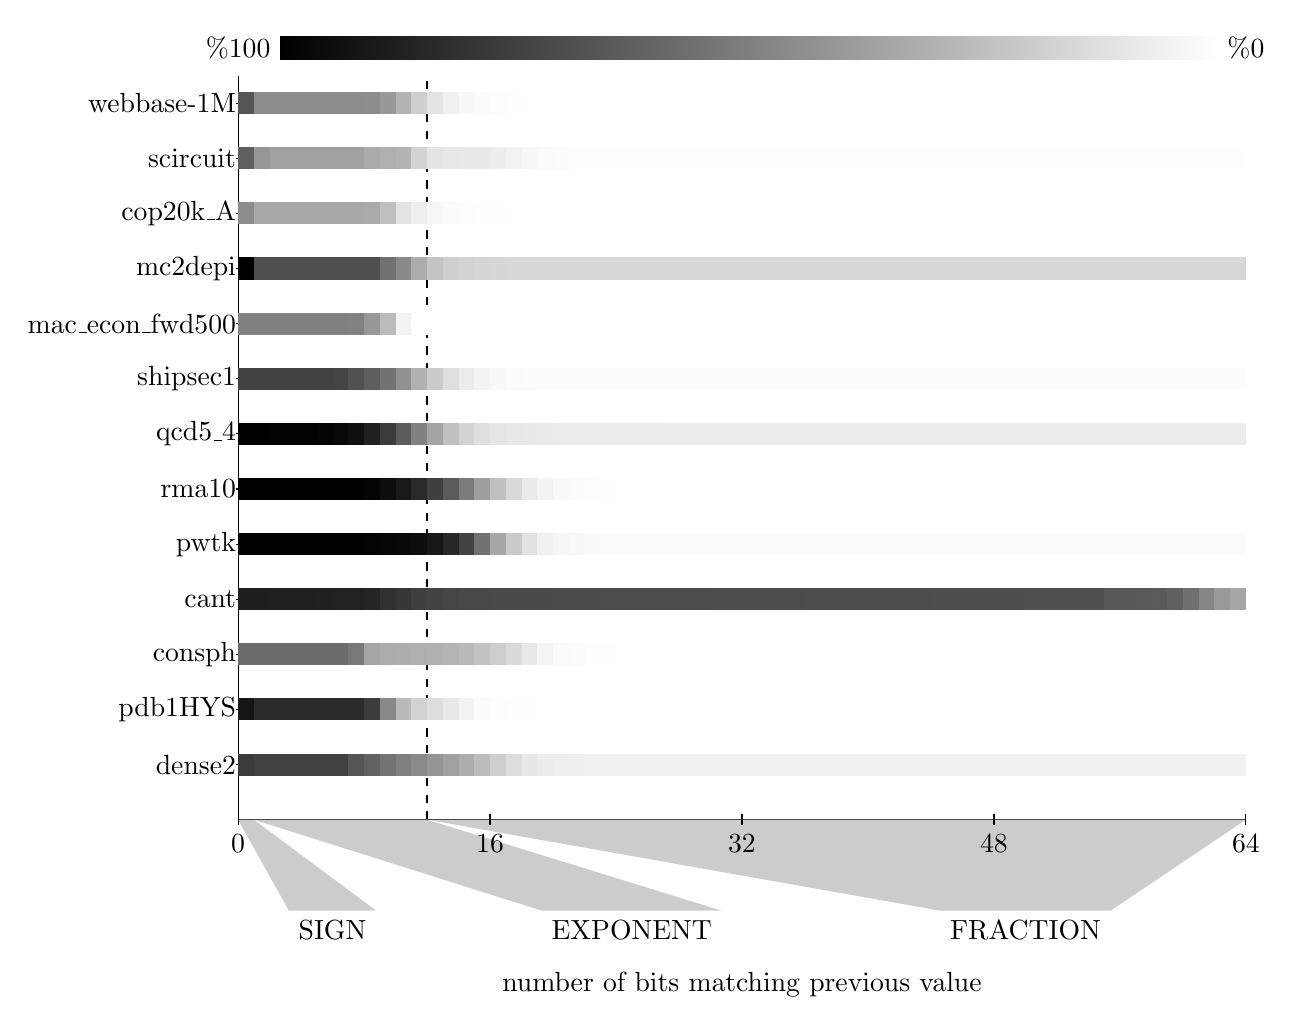
\begin{tikzpicture}[xscale=.2, yscale=.7]
\path[draw] (0,0) -- (64,0);
\path[draw] (0,0) -- (0, 13.5);
\path[draw,dashed] (12,0) -- (12,13.5);
\node(sign) at (6,-2){SIGN};
\node(expo) at (25,-2){EXPONENT};
\node(frac) at (50,-2){FRACTION};
\path[fill=black!20](0,0) -- (1,0) -- (sign.north east) -- (sign.north west) -- cycle;
\path[fill=black!20](1,0) -- (12,0) -- (expo.north east) -- (expo.north west) -- cycle;
\path[fill=black!20](12,0) -- (64,0) -- (frac.north east) -- (frac.north west) -- cycle;

\node[fill=white] at (0,14)(high){\%100};
\node[fill=white] at (64,14)(low){\%0};
\shade[left color=black,right color=white] ([yshift=-.2cm]high.east) rectangle ([yshift=.2cm]low.west);
\foreach \x in {0,16,32,48,64}{
    \draw (\x,.1) -- (\x,-.1)node[anchor=north]{\x};
}

\foreach \n/\y in {dense2/1, pdb1HYS/2, consph/3, cant/4, pwtk/5, rma10/6, qcd5\_4/7, shipsec1/8, mac\_econ\_fwd500/9, mc2depi/10, cop20k\_A/11, scircuit/12, webbase-1M/13}{
    \draw (.1,\y) -- (-.1,\y)node[anchor=east,rotate=0,inner sep=0]{\n};
}
\node at (32,-3) {number of bits matching previous value};

\foreach \xa/\ya/\xb/\yb in {
0/100.00/1/76.93,1/76.93/2/74.42,2/74.42/3/74.41,3/74.41/4/74.41,4/74.41/5/74.41,5/74.41/6/74.41,6/74.41/7/74.41,7/74.41/8/66.79,8/66.79/9/61.45,9/61.45/10/54.39,10/54.39/11/49.91,11/49.91/12/45.95,12/45.95/13/41.70,13/41.70/14/37.33,14/37.33/15/32.39,15/32.39/16/26.28,16/26.28/17/19.34,17/19.34/18/13.25,18/13.25/19/9.29,19/9.29/20/7.47,20/7.47/21/6.62,21/6.62/22/6.22,22/6.22/23/6.03,23/6.03/24/5.93,24/5.93/25/5.88,25/5.88/26/5.86,26/5.86/27/5.85,27/5.85/28/5.84,28/5.84/29/5.84,29/5.84/30/5.84,30/5.84/31/5.84,31/5.84/32/5.84,32/5.84/33/5.84,33/5.84/34/5.84,34/5.84/35/5.84,35/5.84/36/5.84,36/5.84/37/5.84,37/5.84/38/5.84,38/5.84/39/5.84,39/5.84/40/5.84,40/5.84/41/5.84,41/5.84/42/5.84,42/5.84/43/5.84,43/5.84/44/5.84,44/5.84/45/5.84,45/5.84/46/5.84,46/5.84/47/5.84,47/5.84/48/5.84,48/5.84/49/5.84,49/5.84/50/5.84,50/5.84/51/5.84,51/5.84/52/5.84,52/5.84/53/5.84,53/5.84/54/5.84,54/5.84/55/5.84,55/5.84/56/5.84,56/5.84/57/5.84,57/5.84/58/5.84,58/5.84/59/5.84,59/5.84/60/5.84,60/5.84/61/5.84,61/5.84/62/5.84,62/5.84/63/5.84,63/5.84/64/5.84}{
    %\shade[left color=black!\ya, right color=black!\yb] (\xa,0.8) rectangle (\xb,1.2);
    \fill[color=black!\yb] (\xa,0.8) rectangle (\xb,1.2);
}
\foreach \xa/\ya/\xb/\yb in {
0/100.00/1/91.65,1/91.65/2/83.11,2/83.11/3/83.11,3/83.11/4/83.11,4/83.11/5/83.11,5/83.11/6/83.11,6/83.11/7/83.11,7/83.11/8/83.06,8/83.06/9/76.47,9/76.47/10/46.59,10/46.59/11/26.92,11/26.92/12/17.71,12/17.71/13/13.30,13/13.30/14/9.19,14/9.19/15/4.80,15/4.80/16/1.67,16/1.67/17/0.77,17/0.77/18/0.40,18/0.40/19/0.22,19/0.22/20/0.12,20/0.12/21/0.06,21/0.06/22/0.02,22/0.02/23/0.01,23/0.01/24/0.01,24/0.01/25/0.00,25/0.00/26/0.00,26/0.00/27/0.00,27/0.00/28/0.00,28/0.00/29/0.00,29/0.00/30/0.00,30/0.00/31/0.00,31/0.00/32/0.00,32/0.00/33/0.00,33/0.00/34/0.00,34/0.00/35/0.00,35/0.00/36/0.00,36/0.00/37/0.00,37/0.00/38/0.00,38/0.00/39/0.00,39/0.00/40/0.00,40/0.00/41/0.00,41/0.00/42/0.00,42/0.00/43/0.00,43/0.00/44/0.00,44/0.00/45/0.00,45/0.00/46/0.00,46/0.00/47/0.00,47/0.00/48/0.00,48/0.00/49/0.00,49/0.00/50/0.00,50/0.00/51/0.00,51/0.00/52/0.00,52/0.00/53/0.00,53/0.00/54/0.00,54/0.00/55/0.00,55/0.00/56/0.00,56/0.00/57/0.00,57/0.00/58/0.00,58/0.00/59/0.00,59/0.00/60/0.00,60/0.00/61/0.00,61/0.00/62/0.00,62/0.00/63/0.00,63/0.00/64/0.00}{
    %\shade[left color=black!\ya, right color=black!\yb] (\xa,1.8) rectangle (\xb,2.2);
    \fill[color=black!\yb] (\xa,1.8) rectangle (\xb,2.2);
}
\foreach \xa/\ya/\xb/\yb in {
0/100.00/1/58.15,1/58.15/2/58.12,2/58.12/3/58.12,3/58.12/4/58.12,4/58.12/5/58.12,5/58.12/6/58.12,6/58.12/7/58.12,7/58.12/8/53.08,8/53.08/9/35.35,9/35.35/10/32.60,10/32.60/11/32.03,11/32.03/12/31.42,12/31.42/13/30.54,13/30.54/14/29.23,14/29.23/15/27.17,15/27.17/16/24.01,16/24.01/17/19.63,17/19.63/18/14.45,18/14.45/19/8.91,19/8.91/20/4.43,20/4.43/21/1.98,21/1.98/22/0.98,22/0.98/23/0.50,23/0.50/24/0.24,24/0.24/25/0.12,25/0.12/26/0.06,26/0.06/27/0.03,27/0.03/28/0.02,28/0.02/29/0.01,29/0.01/30/0.00,30/0.00/31/0.00,31/0.00/32/0.00,32/0.00/33/0.00,33/0.00/34/0.00,34/0.00/35/0.00,35/0.00/36/0.00,36/0.00/37/0.00,37/0.00/38/0.00,38/0.00/39/0.00,39/0.00/40/0.00,40/0.00/41/0.00,41/0.00/42/0.00,42/0.00/43/0.00,43/0.00/44/0.00,44/0.00/45/0.00,45/0.00/46/0.00,46/0.00/47/0.00,47/0.00/48/0.00,48/0.00/49/0.00,49/0.00/50/0.00,50/0.00/51/0.00,51/0.00/52/0.00,52/0.00/53/0.00,53/0.00/54/0.00,54/0.00/55/0.00,55/0.00/56/0.00,56/0.00/57/0.00,57/0.00/58/0.00,58/0.00/59/0.00,59/0.00/60/0.00,60/0.00/61/0.00,61/0.00/62/0.00,62/0.00/63/0.00,63/0.00/64/0.00}{
    %\shade[left color=black!\ya, right color=black!\yb] (\xa,2.8) rectangle (\xb,3.2);
    \fill[color=black!\yb] (\xa,2.8) rectangle (\xb,3.2);
}
\foreach \xa/\ya/\xb/\yb in {
0/100.00/1/87.91,1/87.91/2/87.89,2/87.89/3/87.63,3/87.63/4/87.62,4/87.62/5/87.42,5/87.42/6/86.91,6/86.91/7/86.86,7/86.86/8/86.78,8/86.78/9/85.62,9/85.62/10/80.89,10/80.89/11/78.75,11/78.75/12/75.68,12/75.68/13/73.61,13/73.61/14/72.53,14/72.53/15/71.95,15/71.95/16/71.66,16/71.66/17/71.50,17/71.50/18/71.37,18/71.37/19/71.32,19/71.32/20/71.19,20/71.19/21/71.07,21/71.07/22/70.93,22/70.93/23/70.81,23/70.81/24/70.72,24/70.72/25/70.66,25/70.66/26/70.61,26/70.61/27/70.58,27/70.58/28/70.52,28/70.52/29/70.48,29/70.48/30/70.41,30/70.41/31/70.35,31/70.35/32/70.27,32/70.27/33/70.21,33/70.21/34/70.16,34/70.16/35/70.09,35/70.09/36/70.04,36/70.04/37/69.98,37/69.98/38/69.91,38/69.91/39/69.86,39/69.86/40/69.82,40/69.82/41/69.78,41/69.78/42/69.74,42/69.74/43/69.68,43/69.68/44/69.63,44/69.63/45/69.57,45/69.57/46/69.52,46/69.52/47/69.46,47/69.46/48/69.40,48/69.40/49/69.33,49/69.33/50/69.28,50/69.28/51/69.21,51/69.21/52/69.16,52/69.16/53/69.08,53/69.08/54/69.01,54/69.01/55/68.90,55/68.90/56/65.88,56/65.88/57/65.71,57/65.71/58/65.29,58/65.29/59/64.89,59/64.89/60/62.45,60/62.45/61/56.00,61/56.00/62/47.50,62/47.50/63/40.14,63/40.14/64/34.83}{
    %\shade[left color=black!\ya, right color=black!\yb] (\xa,3.8) rectangle (\xb,4.2);
    \fill[color=black!\yb] (\xa,3.8) rectangle (\xb,4.2);
}
\foreach \xa/\ya/\xb/\yb in {
0/100.00/1/99.76,1/99.76/2/99.76,2/99.76/3/99.75,3/99.75/4/99.75,4/99.75/5/99.75,5/99.75/6/99.75,6/99.75/7/99.75,7/99.75/8/99.69,8/99.69/9/98.29,9/98.29/10/97.73,10/97.73/11/96.63,11/96.63/12/94.48,12/94.48/13/90.95,13/90.95/14/84.71,14/84.71/15/73.65,15/73.65/16/55.84,16/55.84/17/34.80,17/34.80/18/20.90,18/20.90/19/11.56,19/11.56/20/5.66,20/5.66/21/3.50,21/3.50/22/2.58,22/2.58/23/2.17,23/2.17/24/1.96,24/1.96/25/1.85,25/1.85/26/1.79,26/1.79/27/1.75,27/1.75/28/1.73,28/1.73/29/1.73,29/1.73/30/1.72,30/1.72/31/1.72,31/1.72/32/1.72,32/1.72/33/1.72,33/1.72/34/1.72,34/1.72/35/1.72,35/1.72/36/1.72,36/1.72/37/1.72,37/1.72/38/1.72,38/1.72/39/1.72,39/1.72/40/1.72,40/1.72/41/1.72,41/1.72/42/1.72,42/1.72/43/1.72,43/1.72/44/1.72,44/1.72/45/1.72,45/1.72/46/1.72,46/1.72/47/1.72,47/1.72/48/1.72,48/1.72/49/1.72,49/1.72/50/1.72,50/1.72/51/1.72,51/1.72/52/1.72,52/1.72/53/1.72,53/1.72/54/1.72,54/1.72/55/1.72,55/1.72/56/1.72,56/1.72/57/1.72,57/1.72/58/1.72,58/1.72/59/1.72,59/1.72/60/1.72,60/1.72/61/1.72,61/1.72/62/1.72,62/1.72/63/1.72,63/1.72/64/1.72}{
    %\shade[left color=black!\ya, right color=black!\yb] (\xa,4.8) rectangle (\xb,5.2);
    \fill[color=black!\yb] (\xa,4.8) rectangle (\xb,5.2);
}
\foreach \xa/\ya/\xb/\yb in {
0/100.00/1/100.00,1/100.00/2/99.94,2/99.94/3/99.94,3/99.94/4/99.94,4/99.94/5/99.94,5/99.94/6/99.94,6/99.94/7/99.94,7/99.94/8/99.94,8/99.94/9/98.60,9/98.60/10/94.87,10/94.87/11/90.35,11/90.35/12/83.59,12/83.59/13/75.16,13/75.16/14/64.55,14/64.55/15/51.76,15/51.76/16/37.87,16/37.87/17/25.10,17/25.10/18/15.08,18/15.08/19/8.40,19/8.40/20/4.61,20/4.61/21/2.47,21/2.47/22/1.29,22/1.29/23/0.66,23/0.66/24/0.33,24/0.33/25/0.17,25/0.17/26/0.08,26/0.08/27/0.04,27/0.04/28/0.02,28/0.02/29/0.01,29/0.01/30/0.01,30/0.01/31/0.00,31/0.00/32/0.00,32/0.00/33/0.00,33/0.00/34/0.00,34/0.00/35/0.00,35/0.00/36/0.00,36/0.00/37/0.00,37/0.00/38/0.00,38/0.00/39/0.00,39/0.00/40/0.00,40/0.00/41/0.00,41/0.00/42/0.00,42/0.00/43/0.00,43/0.00/44/0.00,44/0.00/45/0.00,45/0.00/46/0.00,46/0.00/47/0.00,47/0.00/48/0.00,48/0.00/49/0.00,49/0.00/50/0.00,50/0.00/51/0.00,51/0.00/52/0.00,52/0.00/53/0.00,53/0.00/54/0.00,54/0.00/55/0.00,55/0.00/56/0.00,56/0.00/57/0.00,57/0.00/58/0.00,58/0.00/59/0.00,59/0.00/60/0.00,60/0.00/61/0.00,61/0.00/62/0.00,62/0.00/63/0.00,63/0.00/64/0.00}{
    %\shade[left color=black!\ya, right color=black!\yb] (\xa,5.8) rectangle (\xb,6.2);
    \fill[color=black!\yb] (\xa,5.8) rectangle (\xb,6.2);
}
\foreach \xa/\ya/\xb/\yb in {
0/100.00/1/100.00,1/100.00/2/100.00,2/100.00/3/99.20,3/99.20/4/99.20,4/99.20/5/99.20,5/99.20/6/98.55,6/98.55/7/96.95,7/96.95/8/93.65,8/93.65/9/86.97,9/86.97/10/76.57,10/76.57/11/64.09,11/64.09/12/49.36,12/49.36/13/35.74,13/35.74/14/24.84,14/24.84/15/17.33,15/17.33/16/12.71,16/12.71/17/10.33,17/10.33/18/9.15,18/9.15/19/8.54,19/8.54/20/8.21,20/8.21/21/8.03,21/8.03/22/7.92,22/7.92/23/7.85,23/7.85/24/7.80,24/7.80/25/7.75,25/7.75/26/7.71,26/7.71/27/7.67,27/7.67/28/7.64,28/7.64/29/7.60,29/7.60/30/7.57,30/7.57/31/7.53,31/7.53/32/7.49,32/7.49/33/7.47,33/7.47/34/7.41,34/7.41/35/7.36,35/7.36/36/7.36,36/7.36/37/7.36,37/7.36/38/7.36,38/7.36/39/7.36,39/7.36/40/7.36,40/7.36/41/7.36,41/7.36/42/7.36,42/7.36/43/7.36,43/7.36/44/7.36,44/7.36/45/7.36,45/7.36/46/7.36,46/7.36/47/7.36,47/7.36/48/7.36,48/7.36/49/7.36,49/7.36/50/7.36,50/7.36/51/7.36,51/7.36/52/7.36,52/7.36/53/7.36,53/7.36/54/7.36,54/7.36/55/7.36,55/7.36/56/7.36,56/7.36/57/7.36,57/7.36/58/7.36,58/7.36/59/7.36,59/7.36/60/7.36,60/7.36/61/7.36,61/7.36/62/7.36,62/7.36/63/7.36,63/7.36/64/7.36}{
    %\shade[left color=black!\ya, right color=black!\yb] (\xa,6.8) rectangle (\xb,7.2);
    \fill[color=black!\yb] (\xa,6.8) rectangle (\xb,7.2);
}
\foreach \xa/\ya/\xb/\yb in {
0/100.00/1/74.22,1/74.22/2/74.22,2/74.22/3/74.22,3/74.22/4/74.22,4/74.22/5/74.22,5/74.22/6/74.11,6/74.11/7/73.36,7/73.36/8/68.60,8/68.60/9/63.27,9/63.27/10/55.43,10/55.43/11/43.42,11/43.42/12/30.67,12/30.67/13/20.32,13/20.32/14/12.64,14/12.64/15/7.54,15/7.54/16/4.51,16/4.51/17/2.85,17/2.85/18/1.98,18/1.98/19/1.54,19/1.54/20/1.32,20/1.32/21/1.21,21/1.21/22/1.15,22/1.15/23/1.13,23/1.13/24/1.11,24/1.11/25/1.10,25/1.10/26/1.10,26/1.10/27/1.10,27/1.10/28/1.10,28/1.10/29/1.10,29/1.10/30/1.10,30/1.10/31/1.10,31/1.10/32/1.10,32/1.10/33/1.10,33/1.10/34/1.10,34/1.10/35/1.10,35/1.10/36/1.10,36/1.10/37/1.10,37/1.10/38/1.10,38/1.10/39/1.10,39/1.10/40/1.10,40/1.10/41/1.10,41/1.10/42/1.10,42/1.10/43/1.10,43/1.10/44/1.10,44/1.10/45/1.10,45/1.10/46/1.10,46/1.10/47/1.10,47/1.10/48/1.10,48/1.10/49/1.10,49/1.10/50/1.10,50/1.10/51/1.10,51/1.10/52/1.10,52/1.10/53/1.09,53/1.09/54/1.09,54/1.09/55/1.09,55/1.09/56/1.09,56/1.09/57/1.09,57/1.09/58/1.09,58/1.09/59/1.09,59/1.09/60/1.08,60/1.08/61/1.08,61/1.08/62/1.08,62/1.08/63/1.08,63/1.08/64/1.08}{
    %\shade[left color=black!\ya, right color=black!\yb] (\xa,7.8) rectangle (\xb,8.2);
    \fill[color=black!\yb] (\xa,7.8) rectangle (\xb,8.2);
}
\foreach \xa/\ya/\xb/\yb in {
0/100.00/1/49.45,1/49.45/2/49.45,2/49.45/3/49.45,3/49.45/4/49.45,4/49.45/5/49.45,5/49.45/6/49.45,6/49.45/7/49.45,7/49.45/8/49.07,8/49.07/9/40.48,9/40.48/10/26.85,10/26.85/11/4.95,11/4.95/12/0.00,12/0.00/13/0.00,13/0.00/14/0.00,14/0.00/15/0.00,15/0.00/16/0.00,16/0.00/17/0.00,17/0.00/18/0.00,18/0.00/19/0.00,19/0.00/20/0.00,20/0.00/21/0.00,21/0.00/22/0.00,22/0.00/23/0.00,23/0.00/24/0.00,24/0.00/25/0.00,25/0.00/26/0.00,26/0.00/27/0.00,27/0.00/28/0.00,28/0.00/29/0.00,29/0.00/30/0.00,30/0.00/31/0.00,31/0.00/32/0.00,32/0.00/33/0.00,33/0.00/34/0.00,34/0.00/35/0.00,35/0.00/36/0.00,36/0.00/37/0.00,37/0.00/38/0.00,38/0.00/39/0.00,39/0.00/40/0.00,40/0.00/41/0.00,41/0.00/42/0.00,42/0.00/43/0.00,43/0.00/44/0.00,44/0.00/45/0.00,45/0.00/46/0.00,46/0.00/47/0.00,47/0.00/48/0.00,48/0.00/49/0.00,49/0.00/50/0.00,50/0.00/51/0.00,51/0.00/52/0.00,52/0.00/53/0.00,53/0.00/54/0.00,54/0.00/55/0.00,55/0.00/56/0.00,56/0.00/57/0.00,57/0.00/58/0.00,58/0.00/59/0.00,59/0.00/60/0.00,60/0.00/61/0.00,61/0.00/62/0.00,62/0.00/63/0.00,63/0.00/64/0.00}{
    %\shade[left color=black!\ya, right color=black!\yb] (\xa,8.8) rectangle (\xb,9.2);
    \fill[color=black!\yb] (\xa,8.8) rectangle (\xb,9.2);
}
\foreach \xa/\ya/\xb/\yb in {
0/100.00/1/100.00,1/100.00/2/68.91,2/68.91/3/68.91,3/68.91/4/68.91,4/68.91/5/68.91,5/68.91/6/68.91,6/68.91/7/68.91,7/68.91/8/68.91,8/68.91/9/68.91,9/68.91/10/55.65,10/55.65/11/46.40,11/46.40/12/32.54,12/32.54/13/23.22,13/23.22/14/19.01,14/19.01/15/17.35,15/17.35/16/16.46,16/16.46/17/16.00,17/16.00/18/15.76,18/15.76/19/15.64,19/15.64/20/15.59,20/15.59/21/15.55,21/15.55/22/15.54,22/15.54/23/15.53,23/15.53/24/15.53,24/15.53/25/15.52,25/15.52/26/15.52,26/15.52/27/15.52,27/15.52/28/15.52,28/15.52/29/15.52,29/15.52/30/15.52,30/15.52/31/15.52,31/15.52/32/15.52,32/15.52/33/15.52,33/15.52/34/15.52,34/15.52/35/15.52,35/15.52/36/15.52,36/15.52/37/15.52,37/15.52/38/15.52,38/15.52/39/15.52,39/15.52/40/15.52,40/15.52/41/15.52,41/15.52/42/15.52,42/15.52/43/15.52,43/15.52/44/15.52,44/15.52/45/15.52,45/15.52/46/15.52,46/15.52/47/15.52,47/15.52/48/15.52,48/15.52/49/15.52,49/15.52/50/15.52,50/15.52/51/15.52,51/15.52/52/15.52,52/15.52/53/15.52,53/15.52/54/15.52,54/15.52/55/15.52,55/15.52/56/15.52,56/15.52/57/15.52,57/15.52/58/15.52,58/15.52/59/15.52,59/15.52/60/15.52,60/15.52/61/15.52,61/15.52/62/15.52,62/15.52/63/15.52,63/15.52/64/15.52}{
    %\shade[left color=black!\ya, right color=black!\yb] (\xa,9.8) rectangle (\xb,10.2);
    \fill[color=black!\yb] (\xa,9.8) rectangle (\xb,10.2);
}
\foreach \xa/\ya/\xb/\yb in {
0/100.00/1/45.18,1/45.18/2/33.89,2/33.89/3/33.89,3/33.89/4/33.89,4/33.89/5/33.89,5/33.89/6/33.89,6/33.89/7/33.89,7/33.89/8/33.89,8/33.89/9/33.32,9/33.32/10/25.52,10/25.52/11/10.93,11/10.93/12/6.61,12/6.61/13/3.44,13/3.44/14/1.75,14/1.75/15/0.91,15/0.91/16/0.48,16/0.48/17/0.25,17/0.25/18/0.14,18/0.14/19/0.06,19/0.06/20/0.03,20/0.03/21/0.01,21/0.01/22/0.01,22/0.01/23/0.00,23/0.00/24/0.00,24/0.00/25/0.00,25/0.00/26/0.00,26/0.00/27/0.00,27/0.00/28/0.00,28/0.00/29/0.00,29/0.00/30/0.00,30/0.00/31/0.00,31/0.00/32/0.00,32/0.00/33/0.00,33/0.00/34/0.00,34/0.00/35/0.00,35/0.00/36/0.00,36/0.00/37/0.00,37/0.00/38/0.00,38/0.00/39/0.00,39/0.00/40/0.00,40/0.00/41/0.00,41/0.00/42/0.00,42/0.00/43/0.00,43/0.00/44/0.00,44/0.00/45/0.00,45/0.00/46/0.00,46/0.00/47/0.00,47/0.00/48/0.00,48/0.00/49/0.00,49/0.00/50/0.00,50/0.00/51/0.00,51/0.00/52/0.00,52/0.00/53/0.00,53/0.00/54/0.00,54/0.00/55/0.00,55/0.00/56/0.00,56/0.00/57/0.00,57/0.00/58/0.00,58/0.00/59/0.00,59/0.00/60/0.00,60/0.00/61/0.00,61/0.00/62/0.00,62/0.00/63/0.00,63/0.00/64/0.00}{
    %\shade[left color=black!\ya, right color=black!\yb] (\xa,10.8) rectangle (\xb,11.2);
    \fill[color=black!\yb] (\xa,10.8) rectangle (\xb,11.2);
}
\foreach \xa/\ya/\xb/\yb in {
0/100.00/1/62.64,1/62.64/2/41.25,2/41.25/3/36.78,3/36.78/4/36.78,4/36.78/5/36.78,5/36.78/6/36.78,6/36.78/7/36.78,7/36.78/8/36.78,8/36.78/9/33.39,9/33.39/10/31.34,10/31.34/11/29.71,11/29.71/12/17.13,12/17.13/13/10.64,13/10.64/14/9.04,14/9.04/15/8.71,15/8.71/16/8.51,16/8.51/17/6.97,17/6.97/18/4.93,18/4.93/19/3.22,19/3.22/20/1.88,20/1.88/21/1.14,21/1.14/22/0.80,22/0.80/23/0.59,23/0.59/24/0.51,24/0.51/25/0.47,25/0.47/26/0.45,26/0.45/27/0.44,27/0.44/28/0.43,28/0.43/29/0.43,29/0.43/30/0.43,30/0.43/31/0.43,31/0.43/32/0.43,32/0.43/33/0.43,33/0.43/34/0.43,34/0.43/35/0.43,35/0.43/36/0.43,36/0.43/37/0.43,37/0.43/38/0.43,38/0.43/39/0.43,39/0.43/40/0.43,40/0.43/41/0.43,41/0.43/42/0.43,42/0.43/43/0.43,43/0.43/44/0.43,44/0.43/45/0.43,45/0.43/46/0.43,46/0.43/47/0.43,47/0.43/48/0.43,48/0.43/49/0.43,49/0.43/50/0.43,50/0.43/51/0.43,51/0.43/52/0.43,52/0.43/53/0.43,53/0.43/54/0.43,54/0.43/55/0.43,55/0.43/56/0.43,56/0.43/57/0.43,57/0.43/58/0.43,58/0.43/59/0.43,59/0.43/60/0.43,60/0.43/61/0.43,61/0.43/62/0.43,62/0.43/63/0.43,63/0.43/64/0.43}{
    %\shade[left color=black!\ya, right color=black!\yb] (\xa,11.8) rectangle (\xb,12.2);
    \fill[color=black!\yb] (\xa,11.8) rectangle (\xb,12.2);
}
\foreach \xa/\ya/\xb/\yb in {
0/100.00/1/66.51,1/66.51/2/44.98,2/44.98/3/44.98,3/44.98/4/44.98,4/44.98/5/44.98,5/44.98/6/44.98,6/44.98/7/44.98,7/44.98/8/44.98,8/44.98/9/44.67,9/44.67/10/40.39,10/40.39/11/29.85,11/29.85/12/18.76,12/18.76/13/10.86,13/10.86/14/5.72,14/5.72/15/2.90,15/2.90/16/1.45,16/1.45/17/0.72,17/0.72/18/0.36,18/0.36/19/0.18,19/0.18/20/0.09,20/0.09/21/0.05,21/0.05/22/0.02,22/0.02/23/0.01,23/0.01/24/0.01,24/0.01/25/0.00,25/0.00/26/0.00,26/0.00/27/0.00,27/0.00/28/0.00,28/0.00/29/0.00,29/0.00/30/0.00,30/0.00/31/0.00,31/0.00/32/0.00,32/0.00/33/0.00,33/0.00/34/0.00,34/0.00/35/0.00,35/0.00/36/0.00,36/0.00/37/0.00,37/0.00/38/0.00,38/0.00/39/0.00,39/0.00/40/0.00,40/0.00/41/0.00,41/0.00/42/0.00,42/0.00/43/0.00,43/0.00/44/0.00,44/0.00/45/0.00,45/0.00/46/0.00,46/0.00/47/0.00,47/0.00/48/0.00,48/0.00/49/0.00,49/0.00/50/0.00,50/0.00/51/0.00,51/0.00/52/0.00,52/0.00/53/0.00,53/0.00/54/0.00,54/0.00/55/0.00,55/0.00/56/0.00,56/0.00/57/0.00,57/0.00/58/0.00,58/0.00/59/0.00,59/0.00/60/0.00,60/0.00/61/0.00,61/0.00/62/0.00,62/0.00/63/0.00,63/0.00/64/0.00}{
    %\shade[left color=black!\ya, right color=black!\yb] (\xa,12.8) rectangle (\xb,13.2);
    \fill[color=black!\yb] (\xa,12.8) rectangle (\xb,13.2);
}

\end{tikzpicture}
\caption{The above figure represents local prefix prediction. The figure shows the density function of 2 adjacent values sharing at least $x$ number prefix bits. All of the data sets start at $(0,\%100)$. The curves end at the percent of values that are identical to their previous value for that dataset.}
\label{fig:prefix}
\end{figure}%
Datasets might also have repeating patterns of values. For example, the sequence $1.0, 2.0, 3.0, 1.0, 2.0, 3.0$ has an obvious pattern. One can use the Burrows-Wheeler Transform\cite{floatZip:Burrows} to analyze these patterns. \figurename~\ref{fig:bwt} describes this algorithm some, however, many other sources describe this algorithm in more detail\cite{floatZip:Burrows,floatZip:Salomon}. \figurename~\ref{fig:pattern} analyzes the number of repeats that appear after the Burrow-Wheeler Transform. As the figure shows, 4 of the 13 test cases have a lot of patterns, but the rest have relatively few.
\begin{figure}
\center
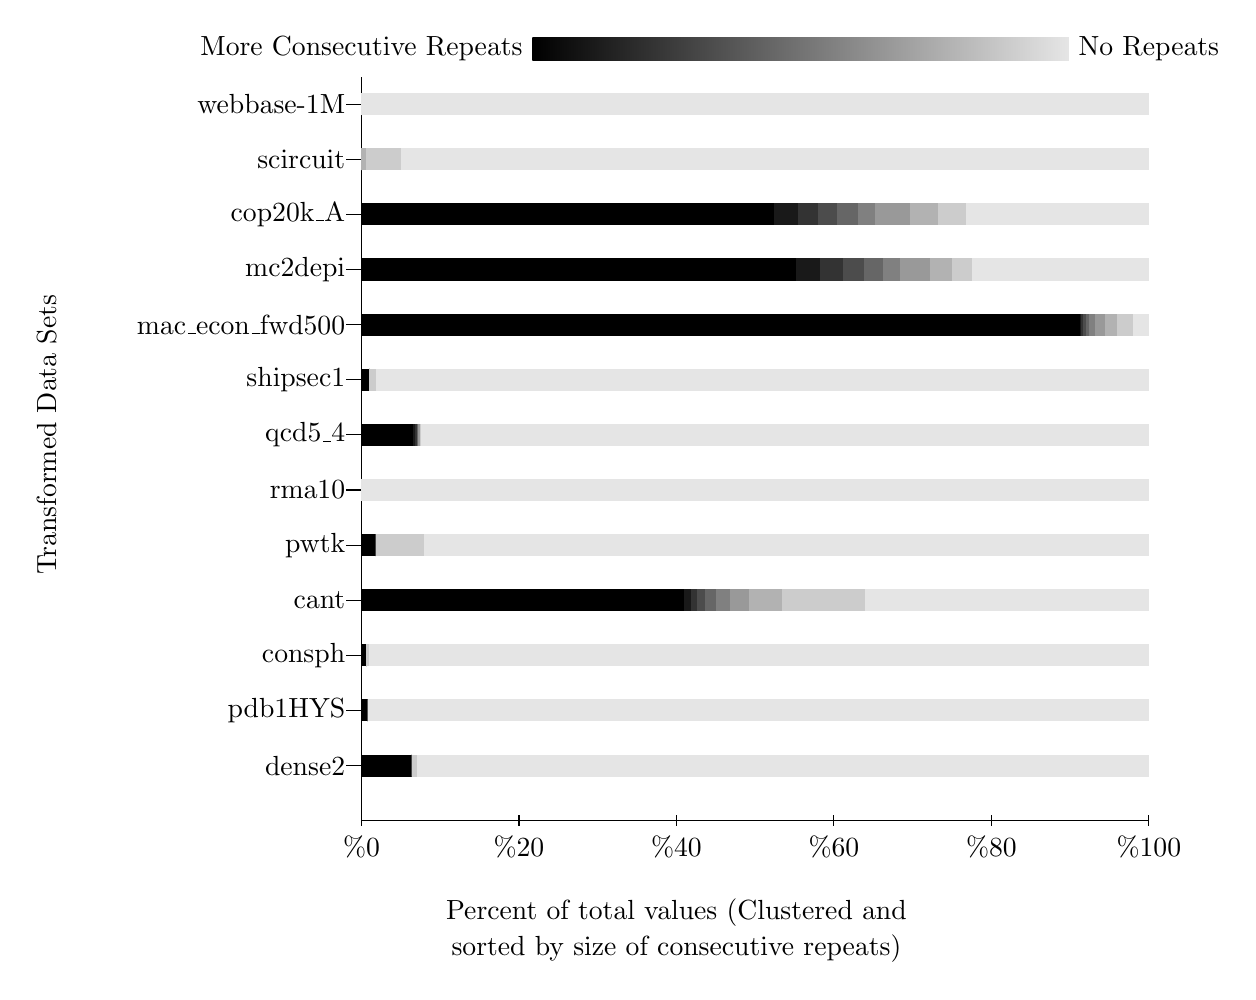
\begin{tikzpicture}[yscale=.7,xscale=2]
\path[draw] (0,0) -- (0,13.5);
\path[draw] (0,0) -- (5,0);
\foreach \x/\v in {0/0,1/20,2/40,3/60,4/80,5/100}{
    \draw (\x,.1) -- (\x,-.1)node[anchor=north]{\%\v};
}
\node[fill=white] at (0,14)(high){More Consecutive Repeats};
\node[fill=white] at (5,14)(low){No Repeats};
\shade[left color=black,right color=black!10] ([yshift=-.2cm]high.east) rectangle ([yshift=.2cm]low.west);

\foreach \n/\y in {dense2/1, pdb1HYS/2, consph/3, cant/4, pwtk/5, rma10/6, qcd5\_4/7, shipsec1/8, mac\_econ\_fwd500/9, mc2depi/10, cop20k\_A/11, scircuit/12, webbase-1M/13}{
    \draw (.1,\y) -- (-.1,\y)node[anchor=east,rotate=0,inner sep=0]{\n};
}
\node at (2,-2){\shortstack{Percent of total values (Clustered and \\sorted by size of consecutive repeats)}};
\node[rotate=90] at (-2,7){Transformed Data Sets};

\foreach \s/\xa/\xb in {
100/0.00/0.32,90/0.32/0.32,80/0.32/0.32,70/0.32/0.32,60/0.32/0.32,50/0.32/0.32,40/0.32/0.32,30/0.32/0.32,20/0.32/0.35,10/0.35/5.00}{
    \fill[black!\s] (\xa,0.8) rectangle (\xb,1.2);
}
\foreach \s/\xa/\xb in {
100/0.00/0.04,90/0.04/0.04,80/0.04/0.04,70/0.04/0.04,60/0.04/0.04,50/0.04/0.04,40/0.04/0.04,30/0.04/0.04,20/0.04/0.04,10/0.04/5.00}{
    \fill[black!\s] (\xa,1.8) rectangle (\xb,2.2);
}
\foreach \s/\xa/\xb in {
100/0.00/0.03,90/0.03/0.03,80/0.03/0.03,70/0.03/0.03,60/0.03/0.03,50/0.03/0.03,40/0.03/0.03,30/0.03/0.03,20/0.03/0.05,10/0.05/5.00}{
    \fill[black!\s] (\xa,2.8) rectangle (\xb,3.2);
}
\foreach \s/\xa/\xb in {
100/0.00/2.05,90/2.05/2.09,80/2.09/2.13,70/2.13/2.18,60/2.18/2.25,50/2.25/2.34,40/2.34/2.46,30/2.46/2.67,20/2.67/3.20,10/3.20/5.00}{
    \fill[black!\s] (\xa,3.8) rectangle (\xb,4.2);
}
\foreach \s/\xa/\xb in {
100/0.00/0.09,90/0.09/0.09,80/0.09/0.09,70/0.09/0.09,60/0.09/0.09,50/0.09/0.09,40/0.09/0.09,30/0.09/0.09,20/0.09/0.40,10/0.40/5.00}{
    \fill[black!\s] (\xa,4.8) rectangle (\xb,5.2);
}
\foreach \s/\xa/\xb in {
100/0.00/0.00,90/0.00/0.00,80/0.00/0.00,70/0.00/0.00,60/0.00/0.00,50/0.00/0.00,40/0.00/0.00,30/0.00/0.00,20/0.00/0.00,10/0.00/5.00}{
    \fill[black!\s] (\xa,5.8) rectangle (\xb,6.2);
}
\foreach \s/\xa/\xb in {
100/0.00/0.33,90/0.33/0.34,80/0.34/0.35,70/0.35/0.35,60/0.35/0.36,50/0.36/0.36,40/0.36/0.37,30/0.37/0.37,20/0.37/0.38,10/0.38/5.00}{
    \fill[black!\s] (\xa,6.8) rectangle (\xb,7.2);
}
\foreach \s/\xa/\xb in {
100/0.00/0.05,90/0.05/0.05,80/0.05/0.05,70/0.05/0.05,60/0.05/0.05,50/0.05/0.05,40/0.05/0.05,30/0.05/0.05,20/0.05/0.09,10/0.09/5.00}{
    \fill[black!\s] (\xa,7.8) rectangle (\xb,8.2);
}
\foreach \s/\xa/\xb in {
100/0.00/4.56,90/4.56/4.57,80/4.57/4.58,70/4.58/4.60,60/4.60/4.62,50/4.62/4.66,40/4.66/4.72,30/4.72/4.80,20/4.80/4.90,10/4.90/5.00}{
    \fill[black!\s] (\xa,8.8) rectangle (\xb,9.2);
}
\foreach \s/\xa/\xb in {
100/0.00/2.76,90/2.76/2.91,80/2.91/3.06,70/3.06/3.19,60/3.19/3.31,50/3.31/3.42,40/3.42/3.61,30/3.61/3.75,20/3.75/3.88,10/3.88/5.00}{
    \fill[black!\s] (\xa,9.8) rectangle (\xb,10.2);
}
\foreach \s/\xa/\xb in {
100/0.00/2.62,90/2.62/2.77,80/2.77/2.90,70/2.90/3.02,60/3.02/3.15,50/3.15/3.26,40/3.26/3.48,30/3.48/3.66,20/3.66/3.84,10/3.84/5.00}{
    \fill[black!\s] (\xa,10.8) rectangle (\xb,11.2);
}
\foreach \s/\xa/\xb in {
100/0.00/0.00,90/0.00/0.00,80/0.00/0.00,70/0.00/0.00,60/0.00/0.00,50/0.00/0.00,40/0.00/0.00,30/0.00/0.03,20/0.03/0.25,10/0.25/5.00}{
    \fill[black!\s] (\xa,11.8) rectangle (\xb,12.2);
}
\foreach \s/\xa/\xb in {
100/0.00/0.00,90/0.00/0.00,80/0.00/0.00,70/0.00/0.00,60/0.00/0.00,50/0.00/0.00,40/0.00/0.00,30/0.00/0.00,20/0.00/0.00,10/0.00/5.00}{
    \fill[black!\s] (\xa,12.8) rectangle (\xb,13.2);
}
%TODO: key
\small
%\node at (2,14) {\shortstack{Percent of values in repeating sequences of length $\geq10$ \tikz \draw[fill=green] (0,0) rectangle (.25,.25);,\\ between $10$ and $1$ \tikz \draw[fill=yellow] (0,0) rectangle (.25,.25);, $=1$ \tikz \draw[fill=red] (0,0) rectangle (.25,.25);}};
\end{tikzpicture}
\caption[not robust]{Pattern analysis using the Burrows-Wheeler Transform. Each shade represents the number of consecutive repeats in a repeating sequence. \tikz{\fill[black] (0,0) rectangle (.25,.25);} represents sequences longer than 9. \tikz \fill[black!50] (0,0) rectangle (.25,.25); represents sequences of length 5. \tikz \fill[black!10] (0,0) rectangle (.25,.25); represents sequences equal to 1 (non-repeating).}
\label{fig:pattern}
\end{figure}

\section{Our Approach}
\label{sec:approach}
Our approach takes advantage of the features in Section \ref{sec:analysis}. The algorithm starts with BWT compression, then compresses further with using prefix and value compression.
\subsection{Burrows-Wheeler Transform Compression}
\indent After completing the Burrows-Wheeler Transform, fzip uses a simple encoding scheme (\figurename~\ref{fig:bwtStep3}). For each value in the BWT, fzip pushes a `0' or `1' onto a bit array to denote whether the value  equals the previous value. If the values differ (a `0' in the bit array) a second array stores the next value. The 4 datasets (msg\_sppm, num\_plasma, obs\_error, obs\_info) expected to do well from the analysis in \figurename~\ref{fig:bwt} do perform well under this compression scheme (see \figurename~\ref{fig:decomp}).
\begin{figure}
\center
\begin{subfigure}{\linewidth}
\center
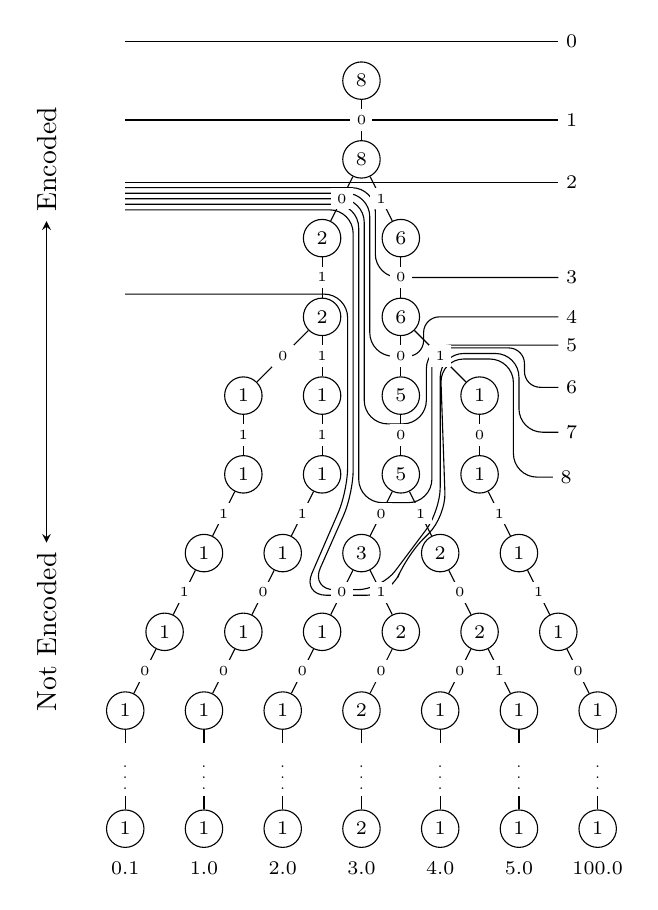
\begin{tikzpicture}
\scriptsize
\node[draw,circle] at (0,0)(n00){8};
%level1
\node[draw,circle] at (0,-1)(n10){8};
%level2
\node[draw,circle] at (-.5,-2)(n20){2};
\node[draw,circle] at (.5,-2)(n21){6};
\node[draw,circle] at (-.5,-3)(n30){2};
\node[draw,circle] at (.5,-3)(n31){6};

\node[draw,circle] at (-1.5,-4)(n40){1};
\node[draw,circle] at (-.5,-4)(n41){1};
\node[draw,circle] at (.5,-4)(n42){5};
\node[draw,circle] at (1.5,-4)(n43){1};

\node[draw,circle] at (-1.5,-5)(n50){1};
\node[draw,circle] at (-.5,-5)(n51){1};
\node[draw,circle] at (.5,-5)(n52){5};
\node[draw,circle] at (1.5,-5)(n53){1};

\node[draw,circle] at (-2,-6)(n60){1};
\node[draw,circle] at (-1,-6)(n61){1};
\node[draw,circle] at (0,-6)(n62){3};
\node[draw,circle] at (1,-6)(n63){2};
\node[draw,circle] at (2,-6)(n64){1};

\node[draw,circle] at (-2.5,-7)(n70){1};
\node[draw,circle] at (-1.5,-7)(n71){1};
\node[draw,circle] at (-0.5,-7)(n72){1};
\node[draw,circle] at (0.5,-7)(n73){2};
\node[draw,circle] at (1.5,-7)(n74){2};
\node[draw,circle] at (2.5,-7)(n75){1};

\node[draw,circle] at (-3,-8)(n80){1};
\node[draw,circle] at (-2,-8)(n81){1};
\node[draw,circle] at (-1, -8)(n82){1};
\node[draw,circle] at (0, -8)(n83){2};
\node[draw,circle] at (1, -8)(n84){1};
\node[draw,circle] at (2, -8)(n85){1};
\node[draw,circle] at (3, -8)(n86){1};

\node[draw,circle] at (-3,-9.5)(n90){1};
\node[draw,circle] at (-2,-9.5)(n91){1};
\node[draw,circle] at (-1,-9.5)(n92){1};
\node[draw,circle] at (0,-9.5)(n93){2};
\node[draw,circle] at (1,-9.5)(n94){1};
\node[draw,circle] at (2,-9.5)(n95){1};
\node[draw,circle] at (3,-9.5)(n96){1};
\scriptsize
\node at (-3,-10){0.1};
\node at (-2,-10){1.0};
\node at (-1,-10){2.0};
\node at (0,-10){3.0};
\node at (1,-10){4.0};
\node at (2,-10){5.0};
\node at (3,-10){100.0};

\scriptsize
\path[draw] (-3,.5) -- (2.5,.5)[anchor=west]node{0};
\path[draw] (-3,-.5) -- (2.5,-.5)[anchor=west]node{1};
\path[draw,yshift=6] (-3,-1.5) -- (2.5,-1.5)[anchor=west]node{2};
%\path[draw,rounded corners=.3cm,yshift=.2cm] (-2.5, -1.5) [shift={(.2cm,.2cm)}] -- (0, -1.5) -- (0,-2.5) -- (2,-2.5);
\path[draw,rounded corners=.3cm,yshift=4] (-3, -1.5) [xshift=5]-- (0, -1.5) [yshift=-4]-- (0,-2.5) [xshift=-5]-- (2.5,-2.5)node[anchor=west]{3};
\path[draw,rounded corners=.3cm,yshift=2] (-3, -1.5) [xshift=3]-- (0, -1.5) [yshift=-2]-- (0,-3.5) [xshift=-9,rounded corners=.2cm] -- (1,-3.5) -- (1,-3) [xshift=6]-- (2.5,-3)node[anchor=west]{4};

\path[draw,rounded corners=.3cm,yshift=0] (-3, -1.5) [xshift=1]-- (0, -1.5) [yshift=4]-- (0,-4.5) [xshift=-6]-- (1,-4.5) -- (1,-3.5) [xshift=5]-- (2.5,-3.5)node[anchor=west]{5};
\path[draw,rounded corners=.3cm,yshift=-2] (-3, -1.5) [xshift=-1]-- (0, -1.5) [yshift=6]-- (0,-5.5) [xshift=-2]-- (1,-5.5) [rounded corners=.2cm,yshift=-1]-- (1,-3.5) [xshift=5]-- (2,-3.5) -- (2,-4) [xshift=-2]-- (2.5,-4)node[anchor=west]{6};
\path[draw,rounded corners=.3cm,yshift=-4] (-3, -1.5) [xshift=-3]-- (0, -1.5) [yshift=-3]-- (0,-5) [shift={(6pt,8pt)}]-- (-.75,-6.5) [xshift=-3]-- (.25,-6.5) -- (1,-5.5) -- (1,-3.5) -- (2,-3.5) -- (2,-4.5) -- (2.5,-4.5)node[anchor=west]{7};
\path[draw,rounded corners=.3cm,yshift=-6] (-3, -2.5) [xshift=-5]-- (0, -2.5) -- (0,-5) [shift={(5pt,5pt)}]-- (-.75,-6.5) [xshift=2]-- (.3,-6.5) -- (.5,-6) -- (1,-5.5) [xshift=-2pt]-- (1,-3.5) [xshift=-2]-- (2,-3.5) -- (2,-5) -- (2.5,-5)node[anchor=west]{8};
%\path[draw,rounded corners=.3cm,yshift=-6] (-3, -1.5) [xshift=-5]-- (0, -1.5) -- (0,-5) [shift={(5pt,5pt)}]-- (-.75,-6.5) -- (0,-6.5) [yshift=1]-- (0,-7.5) [rounded corners=.2cm]-- (1,-7.5) [shift={(2pt,-2pt)}]-- (1,-7) -- (.5,-6) -- (.75,-5.5) [xshift=-2pt]-- (1.5,-5.5) -- (1.5,-6) -- (2,-6)node[anchor=west]{8};

%\path[draw] (-2.5,-8.4) .. controls (-2,-8.4) and (-1.7,-8.3) .. (-1.5,-7.9) -- (0,-5) .. controls (.1,-4.8) and (0,-4.5) .. (1,-4.5) -- (2,-4.5)[anchor=west]node{2};
%\path[draw] (-2.5,-8.5) .. controls (-2,-8.5) and (-1.7,-8.4) .. (-1.5,-8.1) -- (-.2,-5.5) .. controls (0,-5.4) .. (.2,-5.5) -- (.5,-6) .. controls (.8,-6.6) and (.8,-6.5) ..(1.5,-6.5) .. controls (2,-6.5) and (1.5,-5.5) .. (2,-5.5)[anchor=west]node{3};
%\path[draw] (-2.5, -8.6) -- (0,-8.6) .. controls (.1,-8.6) and (.2,-8.6) .. (.5,-8) -- (1,-7) .. controls (1.3,-6.5) and (1,-6.6) ..(2,-6.6)node[anchor=west]{4};
%\path[draw] (-2.5, -8.7) -- (2,-8.7)node[anchor=west]{5};
%\path[draw] (
\tiny
\path[draw] (n00) --node[fill=white]{0} (n10);
\path[draw] (n10) --node[fill=white]{0} (n20);
\path[draw] (n10) --node[fill=white]{1} (n21);
\path[draw] (n20) --node[fill=white]{1} (n30);
\path[draw] (n21) --node[fill=white]{0} (n31);
\path[draw] (n30) --node[fill=white]{0} (n40);
\path[draw] (n30) --node[fill=white]{1} (n41);
\path[draw] (n31) --node[fill=white]{0} (n42);
\path[draw] (n31) --node[fill=white]{1} (n43);

\path[draw] (n40) --node[fill=white]{1} (n50);
\path[draw] (n41) --node[fill=white]{1} (n51);
\path[draw] (n42) --node[fill=white]{0} (n52);
\path[draw] (n43) --node[fill=white]{0} (n53);

\path[draw] (n50) --node[fill=white]{1} (n60);
\path[draw] (n51) --node[fill=white]{1} (n61);
\path[draw] (n52) --node[fill=white]{0} (n62);
\path[draw] (n52) --node[fill=white]{1} (n63);
\path[draw] (n53) --node[fill=white]{1} (n64);

\path[draw] (n60) --node[fill=white]{1} (n70);
\path[draw] (n61) --node[fill=white]{0} (n71);
\path[draw] (n62) --node[fill=white]{0} (n72);
\path[draw] (n62) --node[fill=white]{1} (n73);
\path[draw] (n63) --node[fill=white]{0} (n74);
\path[draw] (n64) --node[fill=white]{1} (n75);

\path[draw] (n70) --node[fill=white]{0} (n80);
\path[draw] (n71) --node[fill=white]{0} (n81);
\path[draw] (n72) --node[fill=white]{0} (n82);
\path[draw] (n73) --node[fill=white]{0} (n83);
\path[draw] (n74) --node[fill=white]{0} (n84);
\path[draw] (n74) --node[fill=white]{1} (n85);
\path[draw] (n75) --node[fill=white]{0} (n86);

\path[draw] (n80) --node[fill=white]{$\vdots$} (n90);
\path[draw] (n81) --node[fill=white]{$\vdots$} (n91);
\path[draw] (n82) --node[fill=white]{$\vdots$} (n92);
\path[draw] (n83) --node[fill=white]{$\vdots$} (n93);
\path[draw] (n84) --node[fill=white]{$\vdots$} (n94);
\path[draw] (n85) --node[fill=white]{$\vdots$} (n95);
\path[draw] (n86) --node[fill=white]{$\vdots$} (n96);

\normalsize
\path (-4,-7)node(ne)[rotate=90]{Not Encoded} -- (-4,-1)node(e)[rotate=90,fill=white]{Encoded};
\path[draw,stealth-stealth] (e)--(ne);
\end{tikzpicture}
\caption{Each node in the above tree represents every prefix that occurs in the dataset.}
\end{subfigure}
\\
\begin{subfigure}{\linewidth}
\center
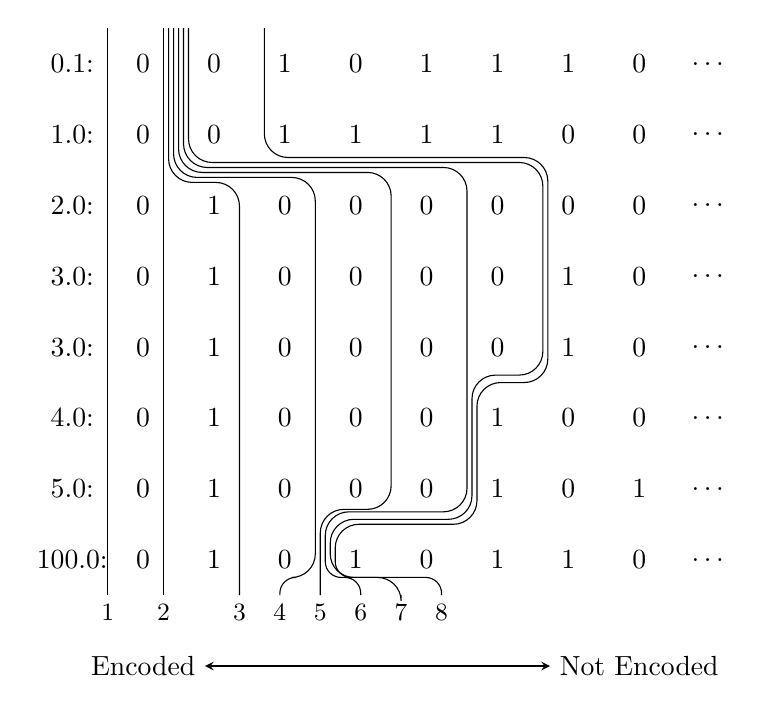
\begin{tikzpicture}[scale=.9]
\node at (0,1){0};\node at (1,1){0};\node at (2,1){1};\node at (3,1){0};\node at (4,1){1};\node at (5,1){1};\node at (6,1){1};\node at (7,1){0};
\node at (0,0){0};\node at (1,0){0};\node at (2,0){1};\node at (3,0){1};\node at (4,0){1};\node at (5,0){1};\node at (6,0){0};\node at (7,0){0};
\node at (0,-1){0};\node at (1,-1){1};\node at (2,-1){0};\node at (3,-1){0};\node at (4,-1){0};\node at (5,-1){0};\node at (6,-1){0};\node at (7,-1){0};
\node at (0,-2){0};\node at (1,-2){1};\node at (2,-2){0};\node at (3,-2){0};\node at (4,-2){0};\node at (5,-2){0};\node at (6,-2){1};\node at (7,-2){0};
\node at (0,-3){0};\node at (1,-3){1};\node at (2,-3){0};\node at (3,-3){0};\node at (4,-3){0};\node at (5,-3){0};\node at (6,-3){1};\node at (7,-3){0};
\node at (0,-4){0};\node at (1,-4){1};\node at (2,-4){0};\node at (3,-4){0};\node at (4,-4){0};\node at (5,-4){1};\node at (6,-4){0};\node at (7,-4){0};
\node at (0,-5){0};\node at (1,-5){1};\node at (2,-5){0};\node at (3,-5){0};\node at (4,-5){0};\node at (5,-5){1};\node at (6,-5){0};\node at (7,-5){1};
\node at (0,-6){0};\node at (1,-6){1};\node at (2,-6){0};\node at (3,-6){1};\node at (4,-6){0};\node at (5,-6){1};\node at (6,-6){1};\node at (7,-6){0};

\node at (8,1){\dots};
\node at (8,0){\dots};
\node at (8,-1){\dots};
\node at (8,-2){\dots};
\node at (8,-3){\dots};
\node at (8,-4){\dots};
\node at (8,-5){\dots};
\node at (8,-6){\dots};

\node at (-1,1){0.1:};\node at (-1,0){1.0:};\node at (-1,-1){2.0:};\node at (-1,-2){3.0:};\node at (-1,-3){3.0:};\node at (-1,-4){4.0:};\node at (-1,-5){5.0:};\node at (-1,-6){100.0:};

\small

\path[draw] (-.5,1.5) -- (-.5,-6.5)node[anchor=north]{1};
\path[draw,xshift=-6] (.5,1.5) -- (.5,-6.5)node[anchor=north]{2};
\path[draw,rounded corners=.3cm,xshift=-4] (.5,1.5) [yshift=-5]-- (.5,-.5) -- (1.5,-.5) [yshift=5]-- (1.5,-6.5)node[anchor=north]{3};
\path[draw,rounded corners=.3cm,xshift=-2] (.5,1.5) [yshift=-3]-- (.5,-.5) -- (2.5,-.5) [yshift=3]-- (2.5,-6.25) [rounded corners=.2cm]-- (2,-6.25) -- (2,-6.5)node[anchor=north]{4};
\path[draw,rounded corners=.3cm,xshift=0] (.5,1.5) [yshift=-1]-- (.5,-.5) -- (3.5,-.5) [yshift=7]-- (3.5,-5.5) -- (2.5,-5.5) [yshift=-6]-- (2.5,-6.5)node[anchor=north]{5};
\path[draw,rounded corners=.3cm,xshift=2] (.5,1.5) [yshift=1]-- (.5,-.5) -- (4.5,-.5) [yshift=4]-- (4.5,-5.5) -- (2.5,-5.5)[rounded corners=.2cm,yshift=-5]-- (2.5,-6.25) -- (3,-6.25) -- (3,-6.5)node[anchor=north]{6};
\path[draw,rounded corners=.3cm,xshift=4] (.5,1.5) [yshift=3]-- (.5,-.5) -- (5.5,-.5) -- (5.5, -3.5) -- (4.5,-3.5) [yshift=-1]-- (4.5,-5.5) -- (2.5,-5.5) [yshift=-2]-- (2.5,-6.25) -- (3.5,-6.25) -- (3.5,-6.5)node[anchor=north]{7};
\path[draw,rounded corners=.3cm,xshift=6] (1.5,1.5) [yshift=5]-- (1.5,-.5) -- (5.5,-.5) [yshift=-5]-- (5.5,-1.5) -- (5.5,-3.5) -- (4.5,-3.5) -- (4.5,-5.5) -- (2.5,-5.5)[rounded corners=.2cm]-- (2.5,-6.25) -- (4,-6.25) -- (4,-6.5)node[anchor=north]{8};
%\path[draw,rounded corners=.3cm,xshift=6] (.5,1.5) [yshift=5]-- (.5,-.5) -- (5.5,-.5) [yshift=-5]-- (5.5,-1.5) -- (6.5,-1.5) -- (6.5, -3.5) -- (4.5,-3.5) [rounded corners=.2cm]-- (4.5,-5.25) -- (5,-5.25) -- (5,-5.5)node[anchor=north]{8};
\normalsize
\path (0,-7.5)node(e){Encoded} -- (7,-7.5)node(ne){Not Encoded};
\path[draw,stealth-stealth] (e)--(ne);
\end{tikzpicture}
\caption{The above sorted list of values gives a second visual representation of how the partition grows.}
\end{subfigure}
\caption{The above 2 figures show the first 8 partition cuts for prefix compression for the example dataset \{0.1, 1.0, 3.0, 5.0, 3.0, 100.0, 4.0, 2.0\}. For simplicity half-precision (16-bit) encoding is used.}
\label{fig:jiles}
\end{figure}
\subsection{Prefix Compression}
After BWT compression, there exists a new array of values. This array should no longer contain many long pattern sequences. However, patterns still exist among the values themselves. The values either repeat or partially repeat. Specifically, many values share common prefixes. fzip uses arithmetic codes to encode these common prefixes.\\
\indent To begin with, fzip creates a large tree to represent all the values in the array. \figurename~\ref{fig:tree} shows an example tree for a small dataset. The tree follows the following rules: each node has up to two children. Each edge represents a 1 bit or a 0 bit. Each node in the tree represents a prefix. The root node represents ``" or no prefix. Each node also has a weight, which represents the number of values with the prefix the node represents. So, the weight of the root node equals the total number of values. The weight of the left (or 0 bit) child of the root represents the prefix ``0". Its weight represents the number of  values that start with ``0" (all non-negative values). Likewise, the right child of the root represents the prefix ``1" and its weight is the number of values starting with 1 (all the negative values).\\

\indent Several properties appear. First, the sum of all the weights of the nodes in any level equals $n$, where $n$ is the total number of values. Moreover, the weight of any set of nodes that partitions the root node from the $65^{th}$ level (and does not contain more nodes than necessary to create the partition) equals $n$.\\
\indent Second, the tree is unbalanced (in our case this is good). Put another way, the datasets contain an unequal number of positive and negative numbers, also any ``normal" dataset would not have an exponential distribution from $2^{-12}$ to $2^{12}$ in such a way to make the rest of the tree balanced.\\
\indent Tree creation starts with the root node, which has a starting weight of 0. To create the rest of the tree, add each value to the tree in the following way: Create a pointer to a ``current node" $c$ and initiate $c$ to the root node. Increment the weight of $c$ (the root node). Then, with the most significant bit (the sign bit) of the floating point value, update $c$ by following the edge that matches this bit. If this edge does not exist create the edge and corresponding node. Then, increment the weight of the new $c$. This repeats until you reach the $64^{th}$ bit. Then, the next value gets added to the tree. This continues until the last value gets added to the tree.\\ 
\indent fzip calculates the prefix codes by creating a partition in the tree. To start, fzip creates a partition with only the root node. Then it includes the edge with the largest cut length in the partition. This repeats until a predetermined number of edges become cut by the partition. Using a list of prefix, prefix code tuples we can represent the encoding scheme of the first 8 partitions of the example in \figurename~\ref{fig:jiles}:\par
\begin{enumerate}
    \item (0,)
    \item (00,0), (01,1)
    \item (00,0), (010,1)
    \item (00,00), (0100,01), (0101,10)
    \item (00,00), (01000,01), (0101,10)
    \item (00,00), (010000,01), (010001,10), (0101,11)
    \item (00,000), (0100000,001), (0100001,010), (010001,011), (0101,100)
    \item (001,000), (0100000,001), (0100001,010), (010001,011), (0101,100)
\end{enumerate} \par
Each added node improves the compression because of the following observation: Let the last added node equal $A$. The number of bits in the uncompressed (not-encoded) stream decreases by weight($A$). However, the code lengths have to increase because the partition cut-size ($k$) increases. The code lengths equal $\textrm{log}_2(k)$. So the increase in the code length equals $\textrm{log}_2(k+1)-\textrm{log}_2(k)$ or $\frac{1}{k}$ by using derivatives. So the codes stream will increase by $\frac{n}{k}$, where $n$ equals to number of values in the data set. If you choose $A$ to maximize $\textrm{weight}(A)$ (a greedy algorithm) then $\textrm{weight}(A) > \textrm{average edge cut} > \frac{n}{k}$. Therefore, the total size of the prefix compression, excluding overhead, keeps improving as the partition increases.\\
\indent But, what if a value occurs often? Say the value $1.0$ occurs $10\%$ of the time? Ideally you should encode $1.0$ as 4 bits ($\textrm{log}_210$ rounded up), but if we continue to grow the partition beyond cutting 16 edges $1.0$ would encode as more than 4 bits. Our solution freezes the codes once a node from the last ($65^{th}$) level becomes included in the partition. This allows fzip to continue to improve prefix compression by growing the partition and also encode common values with shorter codes. This change makes the encoding to variable-length arithmetic encoding.\\
\indent Of course, the overhead to store all of the codes exists. Currently, a 16 byte record describes each code. Each record stores the prefix, the prefix length and the code length. To balance the benefit of prefix encoding with its overhead, we limit the overhead to $1\%$ of the original array size.
\subsection{Repeated Value Extension}
Prefix compression does not compress all of the repeated values. So, fzip extends prefix compression to specifically include all repeated values. Again explaining why repeated values compress well: All of the datasets have less than 37 million values. An index of 26 bits can address the entire dataset. Even if a value repeats only once (occurs twice) there still exists an advantage to store the repeated values in a repeated value array and store the indexes into this array instead of the original values. In the previous example $26+26+64<64+64$ (2 indices plus the value in the array equals less than storing 2 values).\\
\indent To encode these repeats, we expanded the set of prefix codes. This increases the original code lengths by up to one bit. This seemed like a small trade off to make. All the repeats have the same length (64-bits) and the same code length so we can encode each as 8 bytes, instead of the 16 used for the prefixes.

\begin{figure}
\center
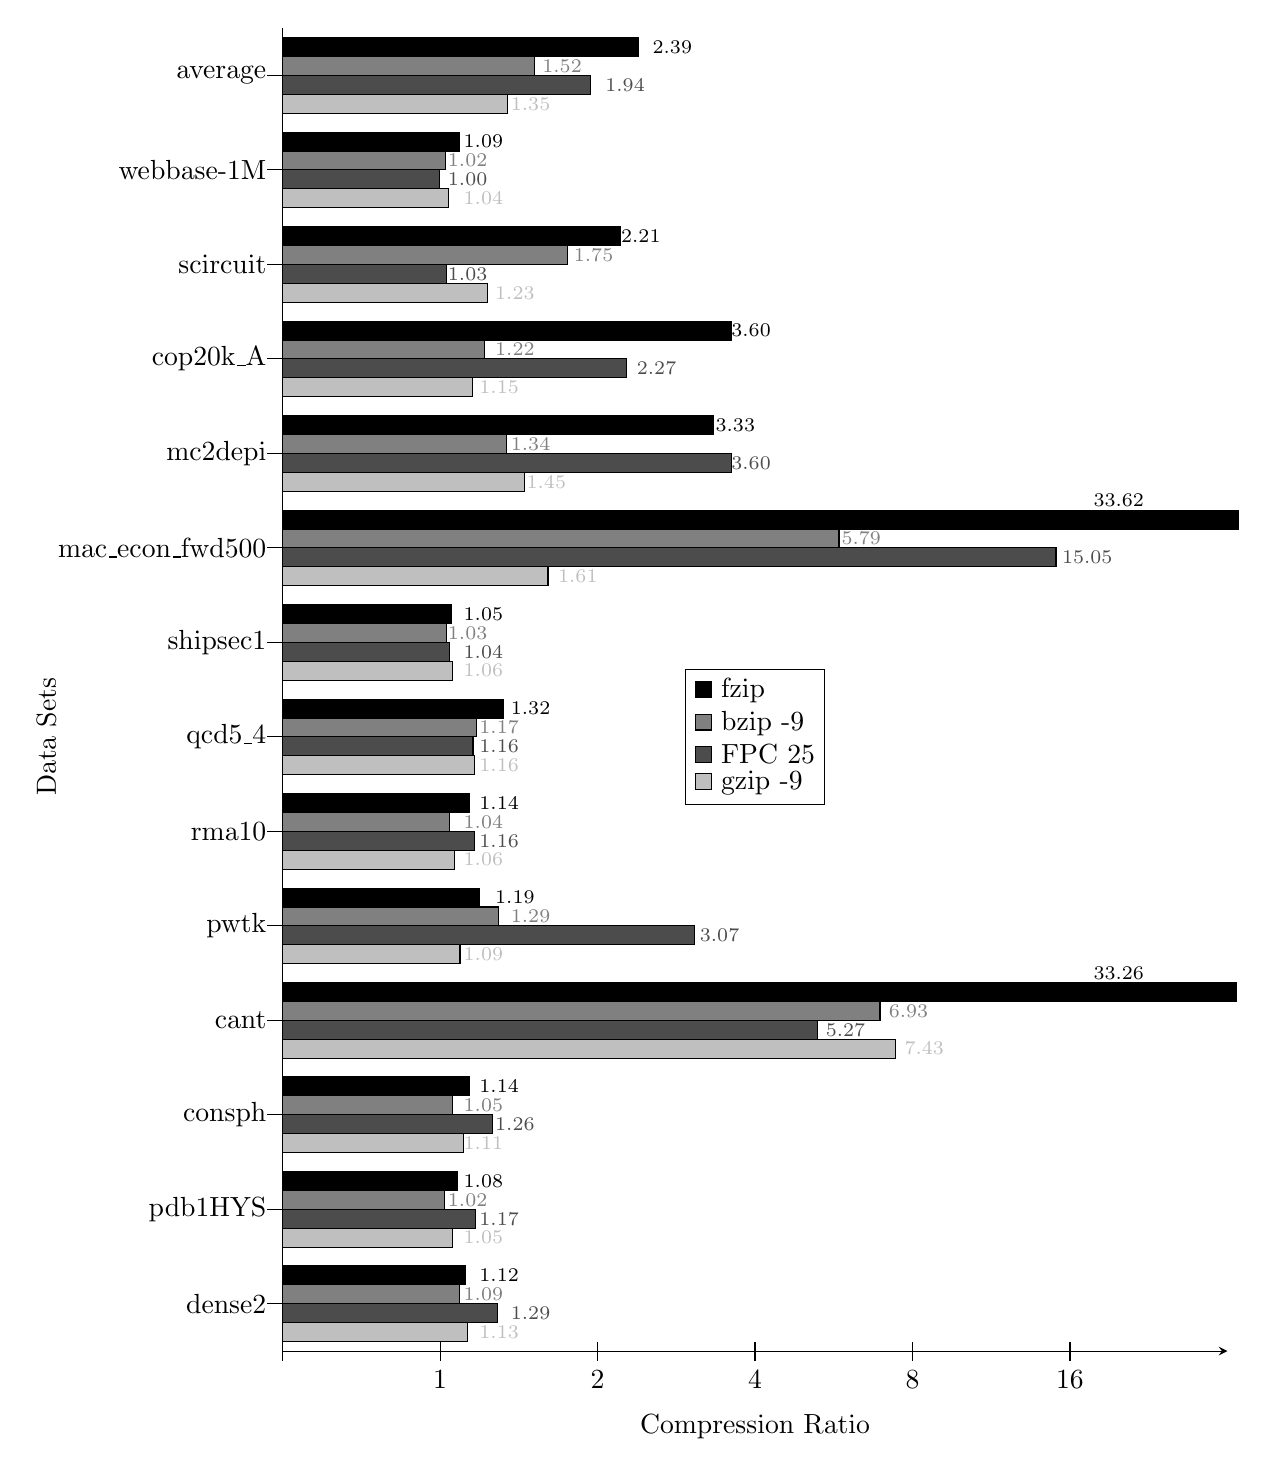
\begin{tikzpicture}[xscale=2,yscale=1.2]
\path[draw] (0,.5) -- (0,14.5);
\path[draw, -stealth] (0,.5) -- (6,.5);
\foreach \x in {0,1,...,5}{
    \path[draw](\x,.4) -- (\x,.6);
}
\foreach \n/\y in {dense2/1, pdb1HYS/2, consph/3, cant/4, pwtk/5, rma10/6, qcd5\_4/7, shipsec1/8, mac\_econ\_fwd500/9, mc2depi/10, cop20k\_A/11, scircuit/12, webbase-1M/13, average/14}{
    \draw (.1,\y) -- (-.1,\y)node[anchor=east,rotate=0,inner sep=0]{\n};
}
\foreach \x/\xscale in {1/1,2/2,3/4,4/8,5/16}{
    \node[anchor=north] at (\x,.4){\xscale};
}
%labels
\node[rotate = 90] at (-1.5,7){Data Sets};
\node at (3, -.3){Compression Ratio};
%TODO: data
%black!50 black!25 black!70 yellow
%fpc
\foreach \y/\val in
{1/1.1763227726404628,2/1.0772429989324603,3/1.1466552221194652,4/3.8935563693054323,5/1.1269728562577654,6/1.0894981508391026,7/1.2166100687424417,8/1.0813396274519387,9/1.6852674065168416,10/1.5340616024211182,11/1.2066432239833953,12/1.2998307618223703,13/1.0510240030244669,14/1.429749850800216}
{
    \draw[fill=black!25] (0,\y-.4) rectangle (\val,\y-.2);
}

\foreach \y/\val in {1/1.3628906426658602,2/1.2252749298695693,3/1.3345682756661328,4/3.398897571202473,5/2.6177686458043974,6/1.2190910582461967,7/1.2091413978385916,8/1.05797006863733,9/4.911499848861109,10/2.8491986517647034,11/2.1826922975161906,12/1.0384361816561078,13/0.9956654097361088,14/1.954568570752994}{
    \draw[fill=black!70] (0,\y-.2) rectangle (\val,\y);
}


\foreach \y/\val in
{1/1.1216785565882526,2/1.0257375614136082,3/1.0772429989324603,4/3.7934797605267003,5/1.3718376173304205,6/1.0607391578576786,7/1.2302030133664215,8/1.0412429822318814,9/3.533314156566792,10/1.4211559606622235,11/1.2833291680516414,12/1.8090027749390862,13/1.034215715337913,14/1.6002697535090047}
{
    \draw[fill=black!50] (0,\y) rectangle (\val,\y+.2);
}

\foreach \y/\val in  {1/1.1634987322828796,2/1.1110313123887439,3/1.189033824390017,4/6.0557162635125446,5/1.250961573533219,6/1.189033824390017,7/1.4005379295837288,8/1.070389327891398,9/6.071247819461443,10/2.735522177296538,11/2.84799690655495,12/2.144046369616707,13/1.1243281350022019,14/2.2579495535311067}{
    \draw[fill=black] (0,\y+.2) rectangle (\val,\y+.4);
}

\scriptsize
\node[black!50,anchor=west] at (1.1,1.1){1.09};
\node[black,anchor=west] at (1.2,1.3){1.12};
\node[black!25,anchor=west] at (1.2,0.7){1.13};
\node[black!70,anchor=west] at (1.4,0.9){1.29};
\node[black!50,anchor=west] at (1.0,2.1){1.02};
\node[black!25,anchor=west] at (1.1,1.7){1.05};
\node[black,anchor=west] at (1.1,2.3){1.08};
\node[black!70,anchor=west] at (1.2,1.9){1.17};
\node[black!50,anchor=west] at (1.1,3.1){1.05};
\node[black!25,anchor=west] at (1.1,2.7){1.11};
\node[black,anchor=west] at (1.2,3.3){1.14};
\node[black!70,anchor=west] at (1.3,2.9){1.26};
\node[black!70,anchor=west] at (3.4,3.9){5.27};
\node[black!50,anchor=west] at (3.8,4.1){6.93};
\node[black!25,anchor=west] at (3.9,3.7){7.43};
\node[black,anchor=west] at (5.1,4.5){33.26};
\node[black!25,anchor=west] at (1.1,4.7){1.09};
\node[black,anchor=west] at (1.3,5.3){1.19};
\node[black!50,anchor=west] at (1.4,5.1){1.29};
\node[black!70,anchor=west] at (2.6,4.9){3.07};
\node[black!50,anchor=west] at (1.1,6.1){1.04};
\node[black!25,anchor=west] at (1.1,5.7){1.06};
\node[black,anchor=west] at (1.2,6.3){1.14};
\node[black!70,anchor=west] at (1.2,5.9){1.16};
\node[black!70,anchor=west] at (1.2,6.9){1.16};
\node[black!25,anchor=west] at (1.2,6.7){1.16};
\node[black!50,anchor=west] at (1.2,7.1){1.17};
\node[black,anchor=west] at (1.4,7.3){1.32};
\node[black!50,anchor=west] at (1.0,8.1){1.03};
\node[black!70,anchor=west] at (1.1,7.9){1.04};
\node[black,anchor=west] at (1.1,8.3){1.05};
\node[black!25,anchor=west] at (1.1,7.7){1.06};
\node[black!25,anchor=west] at (1.7,8.7){1.61};
\node[black!50,anchor=west] at (3.5,9.1){5.79};
\node[black!70,anchor=west] at (4.9,8.9){15.05};
\node[black,anchor=west] at (5.1,9.5){33.62};
\node[black!50,anchor=west] at (1.4,10.1){1.34};
\node[black!25,anchor=west] at (1.5,9.7){1.45};
\node[black,anchor=west] at (2.7,10.3){3.33};
\node[black!70,anchor=west] at (2.8,9.9){3.60};
\node[black!25,anchor=west] at (1.2,10.7){1.15};
\node[black!50,anchor=west] at (1.3,11.1){1.22};
\node[black!70,anchor=west] at (2.2,10.9){2.27};
\node[black,anchor=west] at (2.8,11.3){3.60};
\node[black!70,anchor=west] at (1.0,11.9){1.03};
\node[black!25,anchor=west] at (1.3,11.7){1.23};
\node[black!50,anchor=west] at (1.8,12.1){1.75};
\node[black,anchor=west] at (2.1,12.3){2.21};
\node[black!70,anchor=west] at (1.0,12.9){1.00};
\node[black!50,anchor=west] at (1.0,13.1){1.02};
\node[black!25,anchor=west] at (1.1,12.7){1.04};
\node[black,anchor=west] at (1.1,13.3){1.09};
\node[black!25,anchor=west] at (1.4,13.7){1.35};
\node[black!50,anchor=west] at (1.6,14.1){1.52};
\node[black!70,anchor=west] at (2.0,13.9){1.94};
\node[black,anchor=west] at (2.3,14.3){2.39};


\normalsize
\node[draw] at (3,7){\shortstack[l]{
    \tikz \draw[fill=black] (.1,.1) rectangle (.3,.3); fzip\\
    \tikz \draw[fill=black!50] (.1,.1) rectangle (.3,.3); bzip -9\\
    \tikz \draw[fill=black!70] (.1,.1) rectangle (.3,.3); FPC 25\\
    \tikz \draw[fill=black!25] (.1,.1) rectangle (.3,.3); gzip -9
    }};

\end{tikzpicture}
\caption{The comparison of different compression schemes shows fzip performs quite well.}
\label{fig:compare}
\end{figure}
\begin{figure}
\center
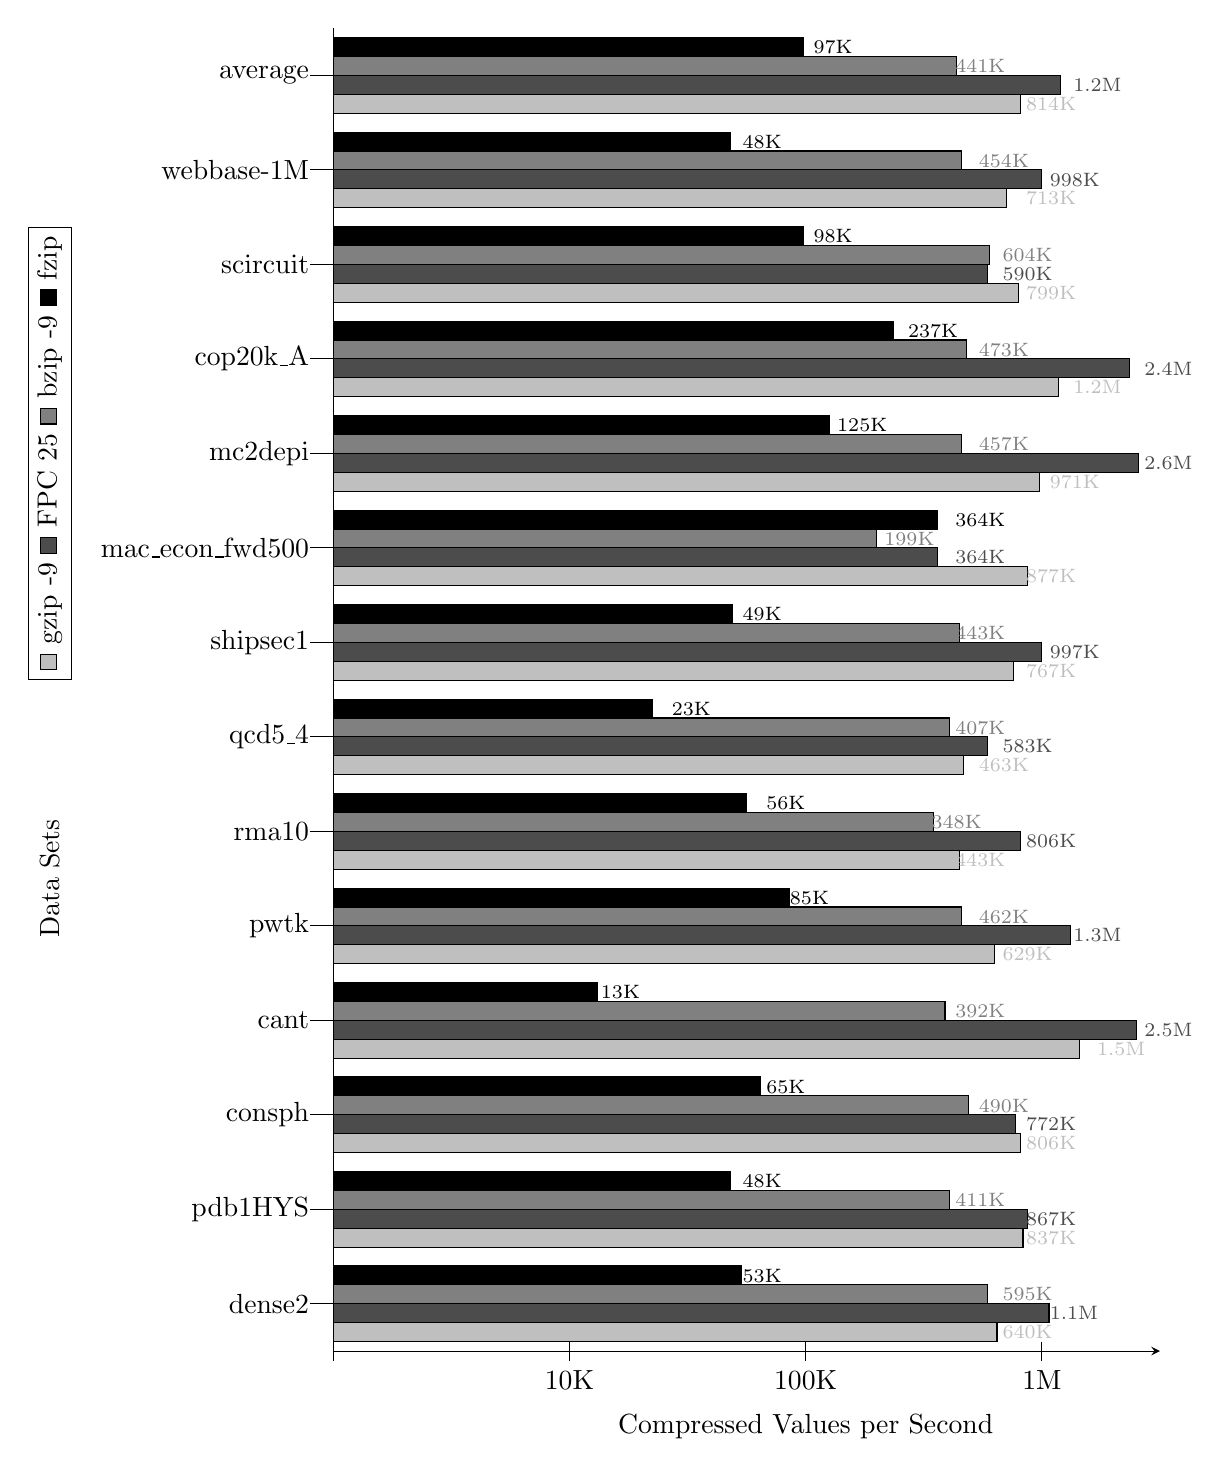
\begin{tikzpicture}[xscale=3, yscale=1.2]
\path[draw, -stealth] (0,.5) -- (3.5,.5);
\path[draw] (0,.5) -- (0,14.5);
\foreach \x in {0,1,...,3}{
    \path[draw](\x,.6) -- (\x,.4);
}
\foreach \n/\y in {dense2/1, pdb1HYS/2, consph/3, cant/4, pwtk/5, rma10/6, qcd5\_4/7, shipsec1/8, mac\_econ\_fwd500/9, mc2depi/10, cop20k\_A/11, scircuit/12, webbase-1M/13, average/14}{
    \draw (.1,\y) -- (-.1,\y)node[anchor=east,rotate=0,inner sep=0]{\n};
}
\foreach \x/\yscale in {1/10K,2/100K,3/1M}{ %,4/10M}{
    \node[anchor=north] at (\x,.4){\yscale};
}

\node[rotate=90] at (-1.2,5.5) {Data Sets};
\node at (2,-.3) {Compressed Values per Second};

\foreach \y/\x in {1/2.81,2/2.92,3/2.91,4/3.16,5/2.80,6/2.65,7/2.67,8/2.88,9/2.94,10/2.99,11/3.07,12/2.90,13/2.85,14/2.91}{
    \draw[rectangle,fill=black!25] (0,\y-.4) rectangle (\x,\y-.2);
}
\foreach \y/\x in {1/3.03,2/2.94,3/2.89,4/3.40,5/3.12,6/2.91,7/2.77,8/3.00,9/2.56,10/3.41,11/3.37,12/2.77,13/3.00,14/3.08}{
    \draw[rectangle,fill=black!70] (0,\y-.2) rectangle (\x,\y);
}
\foreach \y/\x in {1/2.77,2/2.61,3/2.69,4/2.59,5/2.66,6/2.54,7/2.61,8/2.65,9/2.30,10/2.66,11/2.68,12/2.78,13/2.66,14/2.64}{
    \draw[fill=black!50] (0,\y) rectangle (\x,\y+.2);
}
\foreach \y/\x in {1/1.73,2/1.68,3/1.81,4/1.12,5/1.93,6/1.75,7/1.35,8/1.69,9/2.56,10/2.10,11/2.37,12/1.99,13/1.68,14/1.99}{
    \draw[fill=black] (0,\y+.2) rectangle (\x,\y+.4);
}
\scriptsize
\node[black,anchor=west] at (1.7,1.3){53K};
\node[black!50,anchor=west] at (2.8,1.1){595K};
\node[black!25,anchor=west] at (2.8,0.7){640K};
\node[black!70,anchor=west] at (3.0,0.9){1.1M};
\node[black,anchor=west] at (1.7,2.3){48K};
\node[black!50,anchor=west] at (2.6,2.1){411K};
\node[black!25,anchor=west] at (2.9,1.7){837K};
\node[black!70,anchor=west] at (2.9,1.9){867K};
\node[black,anchor=west] at (1.8,3.3){65K};
\node[black!50,anchor=west] at (2.7,3.1){490K};
\node[black!70,anchor=west] at (2.9,2.9){772K};
\node[black!25,anchor=west] at (2.9,2.7){806K};
\node[black,anchor=west] at (1.1,4.3){13K};
\node[black!50,anchor=west] at (2.6,4.1){392K};
\node[black!25,anchor=west] at (3.2,3.7){1.5M};
\node[black!70,anchor=west] at (3.4,3.9){2.5M};
\node[black,anchor=west] at (1.9,5.3){85K};
\node[black!50,anchor=west] at (2.7,5.1){462K};
\node[black!25,anchor=west] at (2.8,4.7){629K};
\node[black!70,anchor=west] at (3.1,4.9){1.3M};
\node[black,anchor=west] at (1.8,6.3){56K};
\node[black!50,anchor=west] at (2.5,6.1){348K};
\node[black!25,anchor=west] at (2.6,5.7){443K};
\node[black!70,anchor=west] at (2.9,5.9){806K};
\node[black,anchor=west] at (1.4,7.3){23K};
\node[black!50,anchor=west] at (2.6,7.1){407K};
\node[black!25,anchor=west] at (2.7,6.7){463K};
\node[black!70,anchor=west] at (2.8,6.9){583K};
\node[black,anchor=west] at (1.7,8.3){49K};
\node[black!50,anchor=west] at (2.6,8.1){443K};
\node[black!25,anchor=west] at (2.9,7.7){767K};
\node[black!70,anchor=west] at (3.0,7.9){997K};
\node[black!50,anchor=west] at (2.3,9.1){199K};
\node[black!70,anchor=west] at (2.6,8.9){364K};
\node[black,anchor=west] at (2.6,9.3){364K};
\node[black!25,anchor=west] at (2.9,8.7){877K};
\node[black,anchor=west] at (2.1,10.3){125K};
\node[black!50,anchor=west] at (2.7,10.1){457K};
\node[black!25,anchor=west] at (3.0,9.7){971K};
\node[black!70,anchor=west] at (3.4,9.9){2.6M};
\node[black,anchor=west] at (2.4,11.3){237K};
\node[black!50,anchor=west] at (2.7,11.1){473K};
\node[black!25,anchor=west] at (3.1,10.7){1.2M};
\node[black!70,anchor=west] at (3.4,10.9){2.4M};
\node[black,anchor=west] at (2.0,12.3){98K};
\node[black!70,anchor=west] at (2.8,11.9){590K};
\node[black!50,anchor=west] at (2.8,12.1){604K};
\node[black!25,anchor=west] at (2.9,11.7){799K};
\node[black,anchor=west] at (1.7,13.3){48K};
\node[black!50,anchor=west] at (2.7,13.1){454K};
\node[black!25,anchor=west] at (2.9,12.7){713K};
\node[black!70,anchor=west] at (3.0,12.9){998K};
\node[black,anchor=west] at (2.0,14.3){97K};
\node[black!50,anchor=west] at (2.6,14.1){441K};
\node[black!25,anchor=west] at (2.9,13.7){814K};
\node[black!70,anchor=west] at (3.1,13.9){1.2M};
\normalsize
\node[draw,rotate=90] at (-1.2,10){\tikz \draw[fill=black!25] (.1,.1) rectangle (.3,.3); gzip -9 \tikz \draw[fill=black!70] (.1,.1) rectangle (.3,.3); FPC 25 \tikz \draw[fill=black!50] (.1,.1) rectangle (.3,.3); bzip -9 \tikz \draw[fill=black] (.1,.1) rectangle (.3,.3); fzip};
\end{tikzpicture}
\caption{The above compression runtime analysis shows that fzip has some improvement to make to compete with other program's runtime.}
\label{fig:runtime}
\end{figure}

\par We did develop Burrows-Wheeler transform compression for fzip, however we do not see this compression as hardware amenable. Our current ideas for taking advantage of repeating patterns include a history table or a hash table.
\section{Disscussion}
We use fzip's results to get an idea of performance. We currently don't have the hardware ameanable version of fzip ready.
